% Cursus Onderzoekstechnieken
%
% Genereer PDF-versie met volgende procedure:
% 
% 1) latexmk -pdf "cursus-onderzoekstechnieken"
% 2) biber "cursus-onderzoekstechnieken"
% 3) latexmk -pdf "cursus-onderzoekstechnieken"
%
\documentclass[11pt,fleqn,a4paper]{book}

%%%%%%%%%%%%%%%%%%%%%%%%%%%%%%%%%%%%%%%%%
% The Legrand Orange Book
% Structural Definitions File
% Version 2.0 (9/2/15)
%
% Original author:
% Mathias Legrand (legrand.mathias@gmail.com) with modifications by:
% Vel (vel@latextemplates.com)
%
% This file has been downloaded from:
% http://www.LaTeXTemplates.com
%
% License:
% CC BY-NC-SA 3.0 (http://creativecommons.org/licenses/by-nc-sa/3.0/)
%
%%%%%%%%%%%%%%%%%%%%%%%%%%%%%%%%%%%%%%%%%

%----------------------------------------------------------------------------------------
%	VARIOUS REQUIRED PACKAGES AND CONFIGURATIONS
%----------------------------------------------------------------------------------------

\usepackage[top=3cm,bottom=3cm,left=3cm,right=3cm,headsep=10pt,a4paper]{geometry} % Page margins
\usepackage[margin=1cm,labelfont=bf]{caption}
\usepackage{graphicx} % Required for including pictures
\graphicspath{{images/}} % Specifies the directory where pictures are stored

\usepackage{titling} % Macros for title, author, etc

\usepackage[toc,page]{appendix}
\usepackage{tikz} % Required for drawing custom shapes
\usepackage{pgfplotstable}
\usepackage{pgfplots}
\pgfplotsset{compat=1.13}
\usetikzlibrary{arrows,shapes,backgrounds,positioning,shadows}
\usetikzlibrary{pgfplots.statistics}

\usepackage[english]{babel} % English language/hyphenation
\usepackage{iflang}

\usepackage{paralist}
\usepackage{enumitem} % Customize lists
\setlist{nolistsep} % Reduce spacing between bullet points and numbered lists

\usepackage{booktabs} % Required for nicer horizontal rules in tables
\usepackage{subcaption}

\usepackage{xcolor} % Required for specifying colors by name
\definecolor{maincolor}{RGB}{0,100,184} % Define the main color used for highlighting throughout the book
\definecolor{hogentblue}{RGB}{0,111,184} % Define the orange color used for highlighting throughout the book

% Paragraph style: no indent, add space between paragraphs
\setlength{\parindent}{0em}
\setlength{\parskip}{1em}

\usepackage{comment} % Gebruikt om oplossingen al dan niet mee te nemen in het compileren

%----------------------------------------------------------------------------------------
%	FONTS
%----------------------------------------------------------------------------------------

\usepackage{avant} % Use the Avantgarde font for headings
%\usepackage{times} % Use the Times font for headings
\usepackage{mathptmx} % Use the Adobe Times Roman as the default text font together with math symbols from the Sym­bol, Chancery and Com­puter Modern fonts
\usepackage{eurosym}

\usepackage{amsfonts}
\usepackage{amsmath}
\usepackage{amssymb}
\usepackage{textcomp}
\usepackage{wasysym}

\usepackage{microtype} % Slightly tweak font spacing for aesthetics
\usepackage[utf8]{inputenc} % Required for including letters with accents
\usepackage[T1]{fontenc} % Use 8-bit encoding that has 256 glyphs

%%============================================================================
%% Colours HoGent corporate identity
%%============================================================================

% Faculty colours
\definecolor{HoGentFBO}{RGB}{0,147,208} % Bedrijf en Organisatie
\definecolor{HoGentFMW}{RGB}{0,168,143} % Mens en Wetenschappen
\definecolor{HoGentFNT}{RGB}{255,0,0}   % Natuur en Techniek
\definecolor{HoGentSoA}{RGB}{0,0,0}     % School of Arts

% Accent colours
\definecolor{HoGentAccent1}{RGB}{0,111,184}   % Dark blue
\definecolor{HoGentAccent2}{RGB}{244,52,69}   % Red
\definecolor{HoGentAccent3}{RGB}{0,156,124}   % Green
\definecolor{HoGentAccent4}{RGB}{239,170,162} % Pink
\definecolor{HoGentAccent5}{RGB}{150,150,150} % Grey
\definecolor{HoGentAccent6}{RGB}{255,218,0}   % Yellow

% Aliases for accent colours
\colorlet{HoGentBlue}{HoGentAccent1}
\colorlet{HoGentRed}{HoGentAccent2}
\colorlet{HoGentGreen}{HoGentAccent3}
\colorlet{HoGentPink}{HoGentAccent4}
\colorlet{HoGentGrey}{HoGentAccent5}
\colorlet{HoGentYellow}{HoGentAccent6}

%------------------------------------------------------------------------------
%	TITLE PAGE
%------------------------------------------------------------------------------

\newcommand{\thetitlepage}{%
\begingroup
\thispagestyle{empty}
\begin{tikzpicture}[remember picture,overlay]
\coordinate [below=12cm] (midpoint) at (current page.north);
\node at (current page.north west)
{\begin{tikzpicture}[remember picture,overlay]
\node[anchor=north west,inner sep=0pt] at (0,0) {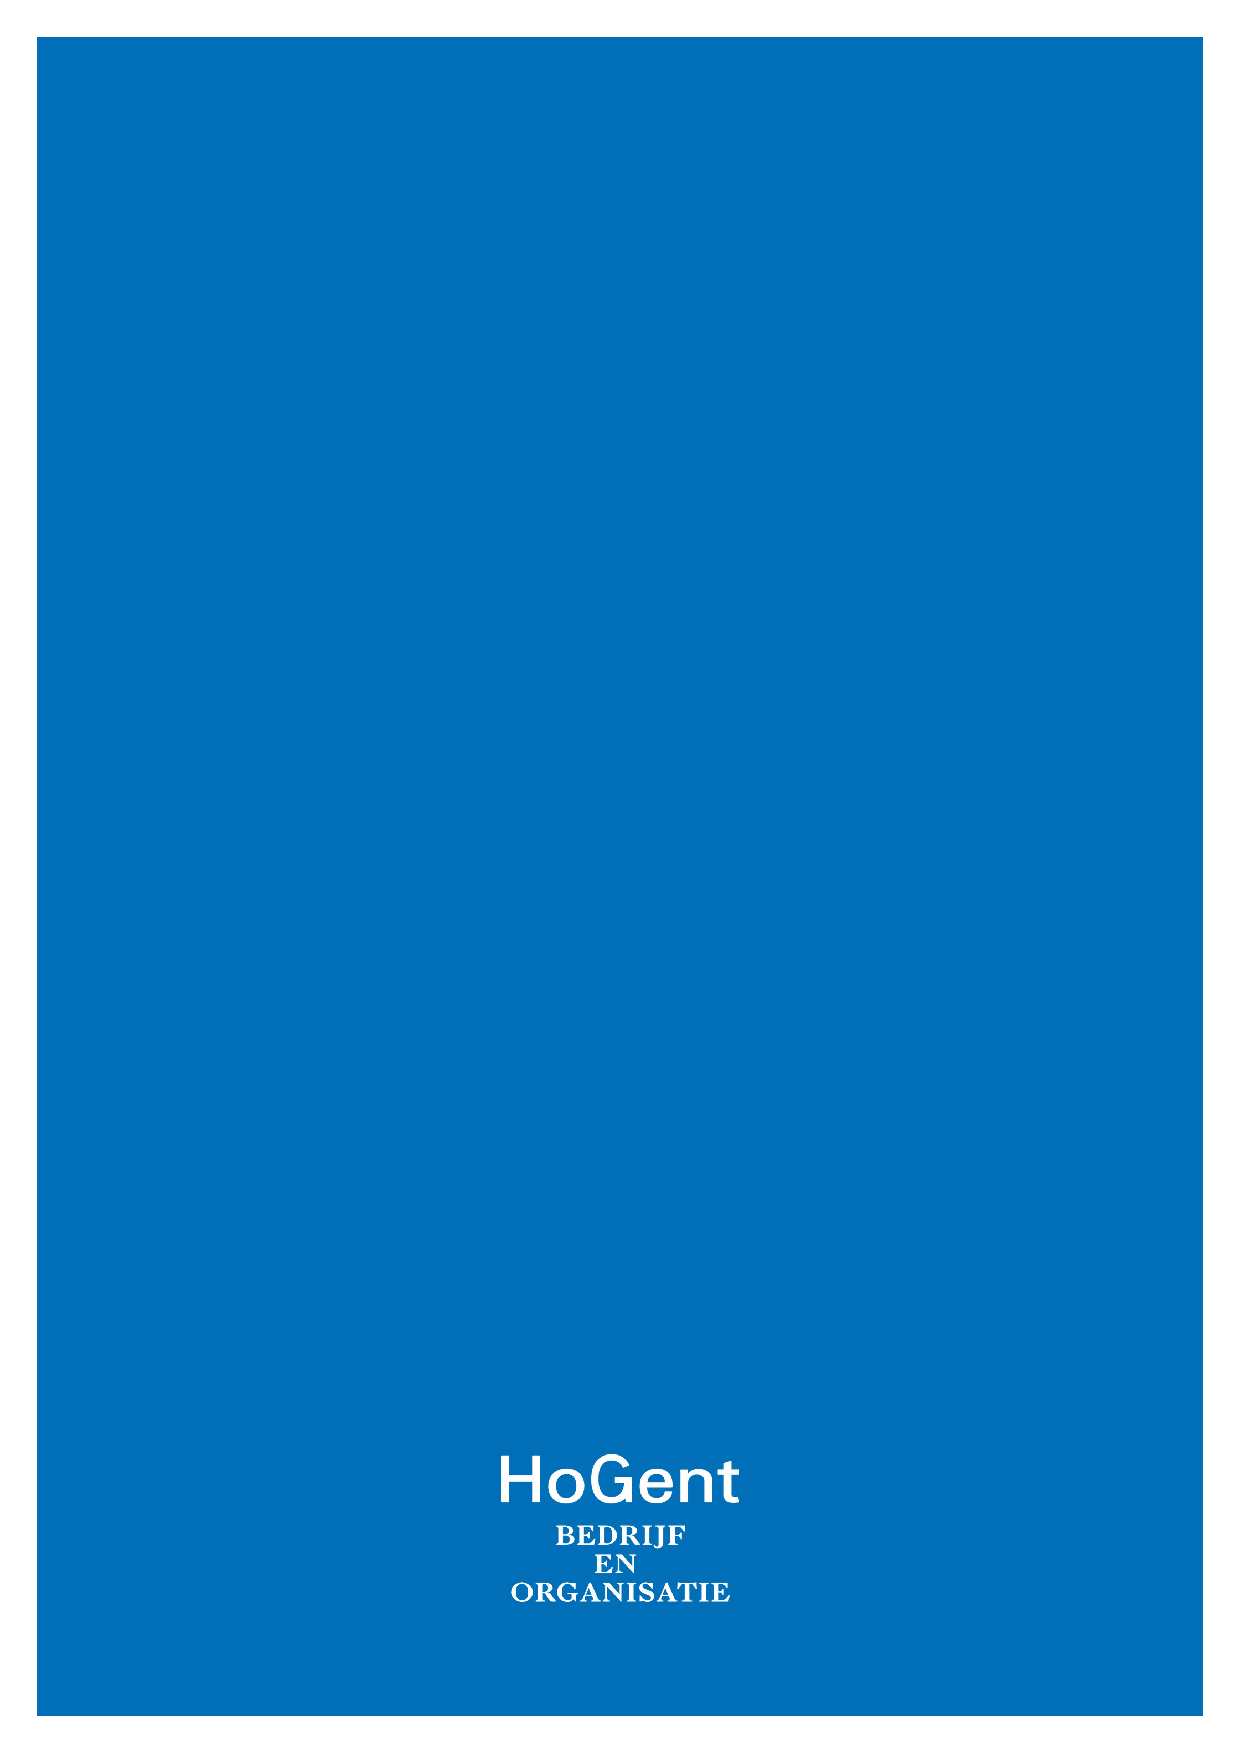
\includegraphics[width=\paperwidth]{background.pdf}}; % Background image
\draw[anchor=north] (midpoint) node [fill=maincolor,fill opacity=0,text=white,text opacity=1,inner sep=1cm]{\Huge\centering\bfseries\sffamily\parbox[c][][t]{\paperwidth}{\centering \thetitle\\[15pt] % Book title
{\Large \thedate}\\[20pt] % Subtitle
{\large \theauthor}}}; % Author name
\end{tikzpicture}};
\end{tikzpicture}
\vfill
\endgroup
}

%----------------------------------------------------------------------------------------
%	BIBLIOGRAPHY AND INDEX
%----------------------------------------------------------------------------------------

\usepackage[style=ieee,backend=biber]{biblatex}
\usepackage{csquotes}
\addbibresource{biblio.bib} % BibTeX bibliography file
\defbibheading{bibempty}{}

\usepackage{calc} % For simpler calculation - used for spacing the index letter headings correctly
\usepackage{makeidx} % Required to make an index
\makeindex % Tells LaTeX to create the files required for indexing

%----------------------------------------------------------------------------------------
%	MAIN TABLE OF CONTENTS
%----------------------------------------------------------------------------------------

\usepackage{titletoc} % Required for manipulating the table of contents

\contentsmargin{0cm} % Removes the default margin

% Part text styling
\titlecontents{part}[0cm]
{\addvspace{20pt}\centering\large\bfseries}
{}
{}
{}

% Chapter text styling
\titlecontents{chapter}[1.25cm] % Indentation
{\addvspace{12pt}\large\sffamily\bfseries} % Spacing and font options for chapters
{\color{maincolor!60}\contentslabel[\Large\thecontentslabel]{1.25cm}\color{maincolor}} % Chapter number
{\color{maincolor}}
{\color{maincolor!60}\normalsize\;\titlerule*[.5pc]{.}\;\thecontentspage} % Page number

% Section text styling
\titlecontents{section}[1.25cm] % Indentation
{\addvspace{3pt}\sffamily\bfseries} % Spacing and font options for sections
{\contentslabel[\thecontentslabel]{1.25cm}} % Section number
{}
{\hfill\color{black}\thecontentspage} % Page number
[]

% Subsection text styling
\titlecontents{subsection}[1.25cm] % Indentation
{\addvspace{1pt}\sffamily\small} % Spacing and font options for subsections
{\contentslabel[\thecontentslabel]{1.25cm}} % Subsection number
{}
{\ \titlerule*[.5pc]{.}\;\thecontentspage} % Page number
[]

% List of figures
\titlecontents{figure}[0em]
{\addvspace{-5pt}\sffamily}
{\thecontentslabel\hspace*{1em}}
{}
{\ \titlerule*[.5pc]{.}\;\thecontentspage}
[]

% List of tables
\titlecontents{table}[0em]
{\addvspace{-5pt}\sffamily}
{\thecontentslabel\hspace*{1em}}
{}
{\ \titlerule*[.5pc]{.}\;\thecontentspage}
[]

%----------------------------------------------------------------------------------------
%	MINI TABLE OF CONTENTS IN PART HEADS
%----------------------------------------------------------------------------------------

% Chapter text styling
\titlecontents{lchapter}[0em] % Indenting
{\addvspace{15pt}\large\sffamily\bfseries} % Spacing and font options for chapters
{\color{maincolor}\contentslabel[\Large\thecontentslabel]{1.25cm}\color{maincolor}} % Chapter number
{}
{\color{maincolor}\normalsize\sffamily\bfseries\;\titlerule*[.5pc]{.}\;\thecontentspage} % Page number

% Section text styling
\titlecontents{lsection}[0em] % Indenting
{\sffamily\small} % Spacing and font options for sections
{\contentslabel[\thecontentslabel]{1.25cm}} % Section number
{}
{}

% Subsection text styling
\titlecontents{lsubsection}[.5em] % Indentation
{\normalfont\footnotesize\sffamily} % Font settings
{}
{}
{}

%----------------------------------------------------------------------------------------
%	PAGE HEADERS
%----------------------------------------------------------------------------------------

\usepackage{fancyhdr} % Required for header and footer configuration

\pagestyle{fancy}
\renewcommand{\chaptermark}[1]{\markboth{\sffamily\normalsize\bfseries\chaptername\ \thechapter.\ #1}{}} % Chapter text font settings
\renewcommand{\sectionmark}[1]{\markright{\sffamily\normalsize\thesection\hspace{5pt}#1}{}} % Section text font settings
\fancyhf{} \fancyhead[LE,RO]{\sffamily\normalsize\thepage} % Font setting for the page number in the header
\fancyhead[LO]{\rightmark} % Print the nearest section name on the left side of odd pages
\fancyhead[RE]{\leftmark} % Print the current chapter name on the right side of even pages
\renewcommand{\headrulewidth}{0.5pt} % Width of the rule under the header
\addtolength{\headheight}{2.5pt} % Increase the spacing around the header slightly
\renewcommand{\footrulewidth}{0pt} % Removes the rule in the footer
\fancypagestyle{plain}{\fancyhead{}\renewcommand{\headrulewidth}{0pt}} % Style for when a plain pagestyle is specified

% Removes the header from odd empty pages at the end of chapters
\makeatletter
\renewcommand{\cleardoublepage}{
\clearpage\ifodd\c@page\else
\hbox{}
\vspace*{\fill}
\thispagestyle{empty}
\newpage
\fi}

%----------------------------------------------------------------------------------------
%	THEOREM STYLES
%----------------------------------------------------------------------------------------

\usepackage{amsmath,amsfonts,amssymb,amsthm} % For math equations, theorems, symbols, etc

\newcommand{\intoo}[2]{\mathopen{]}#1\,;#2\mathclose{[}}
\newcommand{\ud}{\mathop{\mathrm{{}d}}\mathopen{}}
\newcommand{\intff}[2]{\mathopen{[}#1\,;#2\mathclose{]}}
\newtheorem{notation}{Notation}[chapter]

% Boxed/framed environments
\newtheoremstyle{maincolornumbox}% % Theorem style name
{0pt}% Space above
{0pt}% Space below
{\normalfont}% % Body font
{}% Indent amount
{\small\bf\sffamily\color{maincolor}}% % Theorem head font
{\;}% Punctuation after theorem head
{0.25em}% Space after theorem head
{\small\sffamily\color{maincolor}\thmname{#1}\nobreakspace\thmnumber{\@ifnotempty{#1}{}\@upn{#2}}% Theorem text (e.g. Theorem 2.1)
\thmnote{\nobreakspace\the\thm@notefont\sffamily\bfseries\color{black}---\nobreakspace#3.}} % Optional theorem note
\renewcommand{\qedsymbol}{$\blacksquare$}% Optional qed square

\newtheoremstyle{blacknumex}% Theorem style name
{5pt}% Space above
{5pt}% Space below
{\normalfont}% Body font
{} % Indent amount
{\small\bf\sffamily}% Theorem head font
{\;}% Punctuation after theorem head
{0.25em}% Space after theorem head
{\small\sffamily{\tiny\ensuremath{\blacksquare}}\nobreakspace\thmname{#1}\nobreakspace\thmnumber{\@ifnotempty{#1}{}\@upn{#2}}% Theorem text (e.g. Theorem 2.1)
\thmnote{\nobreakspace\the\thm@notefont\sffamily\bfseries---\nobreakspace#3.}}% Optional theorem note

\newtheoremstyle{blacknumbox} % Theorem style name
{0pt}% Space above
{0pt}% Space below
{\normalfont}% Body font
{}% Indent amount
{\small\bf\sffamily}% Theorem head font
{\;}% Punctuation after theorem head
{0.25em}% Space after theorem head
{\small\sffamily\thmname{#1}\nobreakspace\thmnumber{\@ifnotempty{#1}{}\@upn{#2}}% Theorem text (e.g. Theorem 2.1)
\thmnote{\nobreakspace\the\thm@notefont\sffamily\bfseries---\nobreakspace#3.}}% Optional theorem note

% Non-boxed/non-framed environments
\newtheoremstyle{maincolornum}% % Theorem style name
{5pt}% Space above
{5pt}% Space below
{\normalfont}% % Body font
{}% Indent amount
{\small\bf\sffamily\color{maincolor}}% % Theorem head font
{\;}% Punctuation after theorem head
{0.25em}% Space after theorem head
{\small\sffamily\color{maincolor}\thmname{#1}\nobreakspace\thmnumber{\@ifnotempty{#1}{}\@upn{#2}}% Theorem text (e.g. Theorem 2.1)
\thmnote{\nobreakspace\the\thm@notefont\sffamily\bfseries\color{black}---\nobreakspace#3.}} % Optional theorem note
\renewcommand{\qedsymbol}{$\blacksquare$}% Optional qed square
\makeatother

%----------------------------------------------------------------------------------------
%	DEFINITION OF COLORED BOXES
%----------------------------------------------------------------------------------------

\RequirePackage[framemethod=default]{mdframed} % Required for creating the theorem, definition, exercise and corollary boxes

\newcounter{dummy} 
\newtheorem{theoremeT}[dummy]{Stelling}
\newtheorem{problem}{Probleem}[chapter]
\newtheorem{exerciseT}{Oefening}[chapter]
\newtheorem{exampleT}{Voorbeeld}[chapter]
\newtheorem{definitionT}{Definitie}[section]

% Theorem box
\newmdenv[skipabove=7pt,
skipbelow=7pt,
backgroundcolor=black!5,
linecolor=maincolor,
innerleftmargin=5pt,
innerrightmargin=5pt,
innertopmargin=7pt,
innerbottommargin=7pt,
leftmargin=0cm,
rightmargin=0cm,
innerbottommargin=5pt]{tBox}

% Exercise box
\newmdenv[skipabove=7pt,
skipbelow=7pt,
rightline=false,
leftline=true,
topline=false,
bottomline=false,
backgroundcolor=maincolor!10,
linecolor=maincolor,
innerleftmargin=5pt,
innerrightmargin=5pt,
innertopmargin=7pt,
innerbottommargin=7pt,
leftmargin=0cm,
rightmargin=0cm,
linewidth=4pt]{eBox}

% Definition box
\newmdenv[skipabove=7pt,
skipbelow=7pt,
rightline=false,
leftline=true,
topline=false,
bottomline=false,
linecolor=maincolor,
innerleftmargin=5pt,
innerrightmargin=5pt,
innertopmargin=7pt,
innerbottommargin=7pt,
leftmargin=0cm,
rightmargin=0cm,
linewidth=4pt,
innerbottommargin=0pt]{dBox}

% Corollary box
\newmdenv[skipabove=7pt,
skipbelow=7pt,
rightline=false,
leftline=true,
topline=false,
bottomline=false,
linecolor=gray,
backgroundcolor=black!5,
innerleftmargin=5pt,
innerrightmargin=5pt,
innertopmargin=7pt,
innerbottommargin=7pt,
leftmargin=0cm,
rightmargin=0cm,
linewidth=4pt,
innerbottommargin=5pt]{cBox}

% Creates an environment for each type of theorem and assigns it a theorem text style from the "Theorem Styles" section above and a colored box from above
\newenvironment{theorem}{\begin{tBox}\begin{theoremeT}}{\end{theoremeT}\end{tBox}}
\newenvironment{exercise}{\begin{eBox}\begin{exerciseT}}{\hfill{\color{maincolor}\tiny\ensuremath{\blacksquare}}\end{exerciseT}\end{eBox}}
\newenvironment{definition}{\begin{dBox}\begin{definitionT}}{\end{definitionT}\end{dBox}}
\newenvironment{example}{\begin{exampleT}}{\hfill{\tiny\ensuremath{\blacksquare}}\end{exampleT}}
\newenvironment{corollary}{\begin{cBox}\begin{corollaryT}}{\end{corollaryT}\end{cBox}}

%----------------------------------------------------------------------------------------
%	REMARK ENVIRONMENT
%----------------------------------------------------------------------------------------

\newenvironment{remark}{\par\vspace{10pt}\small % Vertical white space above the remark and smaller font size
\begin{list}{}{
\leftmargin=35pt % Indentation on the left
\rightmargin=25pt}\item\ignorespaces % Indentation on the right
\makebox[-2.5pt]{\begin{tikzpicture}[overlay]
\node[draw=maincolor!60,line width=1pt,circle,fill=maincolor!25,font=\sffamily\bfseries,inner sep=2pt,outer sep=0pt] at (-15pt,0pt){\textcolor{maincolor}{R}};\end{tikzpicture}} % Orange R in a circle
\advance\baselineskip -1pt}{\end{list}\vskip5pt} % Tighter line spacing and white space after remark

%----------------------------------------------------------------------------------------
%	SECTION NUMBERING IN THE MARGIN
%----------------------------------------------------------------------------------------

\makeatletter
\renewcommand{\@seccntformat}[1]{\llap{\textcolor{maincolor}{\csname the#1\endcsname}\hspace{1em}}}
\renewcommand{\section}{\@startsection{section}{1}{\z@}
{-4ex \@plus -1ex \@minus -.4ex}
{1ex \@plus.2ex }
{\normalfont\large\sffamily\bfseries}}
\renewcommand{\subsection}{\@startsection {subsection}{2}{\z@}
{-3ex \@plus -0.1ex \@minus -.4ex}
{0.5ex \@plus.2ex }
{\normalfont\sffamily\bfseries}}
\renewcommand{\subsubsection}{\@startsection {subsubsection}{3}{\z@}
{-2ex \@plus -0.1ex \@minus -.2ex}
{.2ex \@plus.2ex }
{\normalfont\small\sffamily\bfseries}}
\renewcommand\paragraph{\@startsection{paragraph}{4}{\z@}
{-2ex \@plus-.2ex \@minus .2ex}
{.1ex}
{\normalfont\small\sffamily\bfseries}}

%----------------------------------------------------------------------------------------
%	PART HEADINGS
%----------------------------------------------------------------------------------------

% numbered part in the table of contents
\newcommand{\@mypartnumtocformat}[2]{%
\setlength\fboxsep{0pt}%
\noindent\colorbox{maincolor!20}{\strut\parbox[c][.7cm]{\ecart}{\color{maincolor!70}\Large\sffamily\bfseries\centering#1}}\hskip\esp\colorbox{maincolor!40}{\strut\parbox[c][.7cm]{\linewidth-\ecart-\esp}{\Large\sffamily\centering#2}}}%
%%%%%%%%%%%%%%%%%%%%%%%%%%%%%%%%%%
% unnumbered part in the table of contents
\newcommand{\@myparttocformat}[1]{%
\setlength\fboxsep{0pt}%
\noindent\colorbox{maincolor!40}{\strut\parbox[c][.7cm]{\linewidth}{\Large\sffamily\centering#1}}}%
%%%%%%%%%%%%%%%%%%%%%%%%%%%%%%%%%%
\newlength\esp
\setlength\esp{4pt}
\newlength\ecart
\setlength\ecart{1.2cm-\esp}
\newcommand{\thepartimage}{}%
\newcommand{\partimage}[1]{\renewcommand{\thepartimage}{#1}}%
\def\@part[#1]#2{%
\ifnum \c@secnumdepth >-2\relax%
\refstepcounter{part}%
\addcontentsline{toc}{part}{\texorpdfstring{\protect\@mypartnumtocformat{\thepart}{#1}}{\partname~\thepart\ ---\ #1}}
\else%
\addcontentsline{toc}{part}{\texorpdfstring{\protect\@myparttocformat{#1}}{#1}}%
\fi%
\startcontents%
\markboth{}{}%
{\thispagestyle{empty}%
\begin{tikzpicture}[remember picture,overlay]%
\node at (current page.north west){\begin{tikzpicture}[remember picture,overlay]%
\fill[maincolor!20](0cm,0cm) rectangle (\paperwidth,-\paperheight);
\node[anchor=north] at (4cm,-3.25cm){\color{maincolor!40}\fontsize{220}{100}\sffamily\bfseries\@Roman\c@part};
\node[anchor=south east] at (\paperwidth-1cm,-\paperheight+1cm){\parbox[t][][t]{8.5cm}{
\printcontents{l}{0}{\setcounter{tocdepth}{1}}%
}};
\node[anchor=north east] at (\paperwidth-1.5cm,-3.25cm){\parbox[t][][t]{15cm}{\strut\raggedleft\color{white}\fontsize{30}{30}\sffamily\bfseries#2}};
\end{tikzpicture}};
\end{tikzpicture}}%
\@endpart}
\def\@spart#1{%
\startcontents%
\phantomsection
{\thispagestyle{empty}%
\begin{tikzpicture}[remember picture,overlay]%
\node at (current page.north west){\begin{tikzpicture}[remember picture,overlay]%
\fill[maincolor!20](0cm,0cm) rectangle (\paperwidth,-\paperheight);
\node[anchor=north east] at (\paperwidth-1.5cm,-3.25cm){\parbox[t][][t]{15cm}{\strut\raggedleft\color{white}\fontsize{30}{30}\sffamily\bfseries#1}};
\end{tikzpicture}};
\end{tikzpicture}}
\addcontentsline{toc}{part}{\texorpdfstring{%
\setlength\fboxsep{0pt}%
\noindent\protect\colorbox{maincolor!40}{\strut\protect\parbox[c][.7cm]{\linewidth}{\Large\sffamily\protect\centering #1\quad\mbox{}}}}{#1}}%
\@endpart}
\def\@endpart{\vfil\newpage
\if@twoside
\if@openright
\null
\thispagestyle{empty}%
\newpage
\fi
\fi
\if@tempswa
\twocolumn
\fi}

%----------------------------------------------------------------------------------------
%	CHAPTER HEADINGS
%----------------------------------------------------------------------------------------

% A switch to conditionally include a picture, implemented by  Christian Hupfer
\newif\ifusechapterimage
\usechapterimagetrue
\newcommand{\thechapterimage}{}%
\newcommand{\chapterimage}[1]{\ifusechapterimage\renewcommand{\thechapterimage}{#1}\fi}%
\def\@makechapterhead#1{%
{\parindent \z@ \raggedright \normalfont
\ifnum \c@secnumdepth >\m@ne
\if@mainmatter
\begin{tikzpicture}[remember picture,overlay]
\node at (current page.north west)
{\begin{tikzpicture}[remember picture,overlay]
\node[anchor=north west,inner sep=0pt] at (0,0) {\ifusechapterimage\includegraphics[width=\paperwidth]{\thechapterimage}\fi};
\draw[anchor=west] (\Gm@lmargin,-9cm) node [line width=2pt,rounded corners=15pt,draw=maincolor,fill=white,fill opacity=0.5,inner sep=15pt]{\strut\makebox[22cm]{}};
\draw[anchor=west] (\Gm@lmargin+.3cm,-9cm) node {\huge\sffamily\bfseries\color{black}\thechapter. #1\strut};
\end{tikzpicture}};
\end{tikzpicture}
\else
\begin{tikzpicture}[remember picture,overlay]
\node at (current page.north west)
{\begin{tikzpicture}[remember picture,overlay]
\node[anchor=north west,inner sep=0pt] at (0,0) {\ifusechapterimage\includegraphics[width=\paperwidth]{\thechapterimage}\fi};
\draw[anchor=west] (\Gm@lmargin,-9cm) node [line width=2pt,rounded corners=15pt,draw=maincolor,fill=white,fill opacity=0.5,inner sep=15pt]{\strut\makebox[22cm]{}};
\draw[anchor=west] (\Gm@lmargin+.3cm,-9cm) node {\huge\sffamily\bfseries\color{black}#1\strut};
\end{tikzpicture}};
\end{tikzpicture}
\fi\fi\par\vspace*{270\p@}}}

%-------------------------------------------

\def\@makeschapterhead#1{%
\begin{tikzpicture}[remember picture,overlay]
\node at (current page.north west)
{\begin{tikzpicture}[remember picture,overlay]
\node[anchor=north west,inner sep=0pt] at (0,0) {\ifusechapterimage\includegraphics[width=\paperwidth]{\thechapterimage}\fi};
\draw[anchor=west] (\Gm@lmargin,-9cm) node [line width=2pt,rounded corners=15pt,draw=maincolor,fill=white,fill opacity=0.5,inner sep=15pt]{\strut\makebox[22cm]{}};
\draw[anchor=west] (\Gm@lmargin+.3cm,-9cm) node {\huge\sffamily\bfseries\color{black}#1\strut};
\end{tikzpicture}};
\end{tikzpicture}
\par\vspace*{270\p@}}
\makeatother

%----------------------------------------------------------------------------------------
%	HYPERLINKS IN THE DOCUMENTS
%----------------------------------------------------------------------------------------

\usepackage{hyperref}
\hypersetup{hidelinks,colorlinks=false,breaklinks=true,urlcolor= maincolor,bookmarksopen=false,pdftitle={Title},pdfauthor={Author}}
\usepackage{bookmark}
\bookmarksetup{
open,
numbered,
addtohook={%
\ifnum\bookmarkget{level}=0 % chapter
\bookmarksetup{bold}%
\fi
\ifnum\bookmarkget{level}=-1 % part
\bookmarksetup{color=maincolor,bold}%
\fi
}
}

%----------------------------------------------------------------------------------------
%	Math stuff
%----------------------------------------------------------------------------------------

\pgfmathdeclarefunction{gauss}{2}{%
	\pgfmathparse{1/(#2*sqrt(2*pi))*exp(-((x-#1)^2)/(2*#2^2))}%
}

\def\R{\mathbb{R}}

%----------------------------------------------------------------------------------------
%	Format R code
%----------------------------------------------------------------------------------------
\usepackage{listings}

\lstset{ %
  language=Java,                     % the language of the code
  inputencoding=utf8,             % Allow (some) Unicode characters in the code
  extendedchars=true,
  literate={é}{{\'e}}1 {ë}{{\"e}}1 {è}{{\`e}}1 {á}{{\'a}}1 {à}{{\`a}}1 {ó}{{\'o}}1 {ò}{{\`o}}1 {²}{{$^2$}}1 {€}{{\euro}}1,
  basicstyle=\normalsize,       % the size of the fonts that are used for the code
  numbers=left,                   % where to put the line-numbers
  numberstyle=\tiny\color{gray},  % the style that is used for the line-numbers
  stepnumber=1,                   % the step between two line-numbers. If it's 1, each line
  % will be numbered
  numbersep=5pt,                  % how far the line-numbers are from the code
  backgroundcolor=\color{white},  % choose the background color. You must add \usepackage{color}
  showspaces=false,               % show spaces adding particular underscores
  showstringspaces=false,         % underline spaces within strings
  showtabs=false,                 % show tabs within strings adding particular underscores
  frame=single,                   % adds a frame around the code
  rulecolor=\color{black},        % if not set, the frame-color may be changed on line-breaks within not-black text (e.g. commens (green here))
  tabsize=2,                      % sets default tabsize to 2 spaces
  captionpos=b,                   % sets the caption-position to bottom
  breaklines=true,                % sets automatic line breaking
  breakatwhitespace=false,        % sets if automatic breaks should only happen at whitespace
  keywordstyle=\color{HoGentBlue},      % keyword style
  commentstyle=\color{HoGentGrey},   % comment style
  stringstyle=\color{HoGentRed},      % string literal style
  morekeywords={*,...}            % if you want to add more keywords to the set
}



\author{Dr. Jens Buysse, Karine Samyn}
\title{Native Apps 1: Android}
\date{2017-2018}

\begin{document}

\thetitlepage

%----------------------------------------------------------------------------------------
%	COPYRIGHT PAGE
%----------------------------------------------------------------------------------------

\newpage
~\vfill
\thispagestyle{empty}

\noindent Copyright \copyright\ 2017-2017 Jens Buysse\\ % Copyright notice

\noindent \textsc{www.hogent.be}\\ % URL

\noindent \textit{Generated on \today} % Printing/edition date

%----------------------------------------------------------------------------------------
%	TABLE OF CONTENTS
%----------------------------------------------------------------------------------------

\chapterimage{images/chapterhead1.jpg}

\tableofcontents % Print the table of contents itself

\cleardoublepage % Forces the first chapter to start on an odd page so it's on the right

\setlength{\parindent}{0pt}

\includecomment{solution}
%\excludecomment{solution}
I would like to thank Karine Samyn for reviewing the course material. 

And for the time being, I wish you a lot of fun reading and studying this course!

\begin{flushright}
	-- Jens Buysse
\end{flushright}

\chapter{About this course}

\section{Introduction}
This course is an introduction into the wonderful world of Android.
The aim of this course is not to turn you into a specialized Android developer, but to give an introduction to the general concepts of the Android framework and provide the tools you need to find your way in this fragmented world. 

Starting from first semester of 2018 we will adopt Kotlin as the default language for developing Android applications. 

\section{ECTS}
ECTS is an acronym for European Credit Transfer and Accumulation System.
This stipulates every final attainment level you should have when finishing this course.
These can be found \href{https://bamaflexweb.hogent.be/BMFUIDetailxOLOD.aspx?a=98522\&b=5\&c=1}{here}. 

\section{Course Material}
The course is taught using the following materials:

\begin{itemize}
	\item These course notes
	\item Book \textit{Kotlin for Android Developers} \cite{Leiva2018}
	\item Book  \textit{The Busy Coder's Guide to Android Development} \cite{murphymarkl.2017}
	\item External resources and references (these course notes, Chamilo links \dots)
	\item TODO: boeken toevoegen die we gebruikt hebben
\end{itemize}

\section{Course organisation}
This course consists of 12 lessons.
The first part of each lesson will cover the theoretical aspects and the second part will put theory into practice.
Normally you will not be able to complete the exercises in one hour so it is up to you to complete these exercises at home.
If you encounter any difficulties  you are welcome to ask questions in the next lesson or via the forum on Chamilo.
We don't encourage sending personal e-mail: you are not alone in having difficulties with certain topics.
E-mail is not the best way for us to help you.

Think carefully when you write down your question: make it reproducible. Follow these guidelines: \href{https://stackoverflow.com/help/how-to-ask}{https://stackoverflow.com/help/how-to-ask}

\subsection{Covered Topics}
This course will roughly cover the following topics:

\begin{enumerate}
	\item History of  Android and Intro Kotlin
	\item Activities + layout files 
	\item Structure of an  app, Activity lifecycle, Resources, buildproces
	\item Fragments + UI components and layouts 
	\item Intents, BroadcastReceivers (EventBus) and Parcable 
	\item recyclerview + cardview 
	\item Android coding practices  + common Android software architectures  
	\item Persistentence in Android
	\item Networking
	\item Testing in Android
	\item Composer for android testing
	\item Memory leaks 
	\item Firebase 
\end{enumerate}

\section{Prior knowledge}
This course assumes knowledge of the Java programming language.
You do not need to know everything, but you need to understand the following concepts:

\begin{itemize}
	\item Language fundamentals (flow control, etc.)
	\item Classes and objects
	\item Methods and data members
	\item Public, private, and protected
	\item Static and instance scope
	\item Exceptions
	\item Threads
	\item Collections
	\item Generics
	\item File I/O
	\item Reflection
	\item Interfaces
\end{itemize}

\section{Examination}
Both for the first as for the second exam period, you will be examined via an oral exam.
You will be handed a set of questions and  you will have time to prepare them.
Some of the questions will be regarding the exercises you have made during the year, so you are obliged to have made them all.
\textbf{If your question is one regarding an exercise you have not made, you will receive a 0 on that question.}

Working together on the exercises is encouraged, but make sure that you have written all the code yourself.
You will get some hard questions and it is very difficult to explain code that isn't yours.
Document your code well and make sure you remember why you have written it the way you have.



\chapterimage{images/hellochapterhead.jpg}

\chapter{Hello Android}
Android\cite{Todd2017} is a mobile operating system which is found on a variety of modern devices, the most popular being smartphones. On top of that, you will also find Android on tablets, TV streaming boxes and other portable gadgets.

Android is basically a piece of software which allows your hardware to function. The Android OS gives you access to apps, including many of Google's own creation. These allow you to look for information on the web, play music and videos, check your location on a map, take photos using your device's camera and plenty more besides.

\section{Open source Android}
Android has open source roots. The project began under Android, Inc. in 2005, which Google bought two years later. That same year, Google and several other companies formed  \footnote{The Open Handset Alliance is a group of 84 technology and mobile companies who have come together to accelerate innovation in mobile and offer consumers a richer, less expensive, and better mobile experience. They have developed Android, the first complete, open, and free mobile platform.}{Open Handset Alliance} \cite{alliance}, with Android being the primary piece of software this consortium is built on.

Android is based on the Linux kernel where most parts are open source with a few binary blobs included to make things work with certain hardware. The core Android platform, known as the Android Open Source Project (AOSP), is available for anyone to do with what they wish.

But is it realy open source ? For the most part, Google develops Android. Once or twice a year, the company dumps  new code over a metaphorical wall that tinkerers and hardware makers use to put in their own code. This is in contrast with many other well-known open source projects : they typically seek more involvement from the broader community. Red Hat may fund a good portion of the work that goes into GNOME, but developers from all over the world contribute code. By comparison, Android comes off as entirely a Google product.



\section{Android version \& updates}
Google is constantly working on new versions of the Android software. These releases are infrequent; at the moment Google is releasing a big Android update once a year.

Versions usually come with a numerical code and a name that’s so far been themed after sweets and desserts, running in alphabetical order.

\begin{description}
	\item[Android 1.5]  Cupcake
	\item[Android 1.6]  Donut
	\item[Android 2.1]  Eclair
	\item[Android 2.2]  Froyo
	\item[Android 2.3]  Gingerbread
	\item[Android 3.2 Honeycomb]  - The first OS design specifically for tablets, launching on the Motorola Xoom
	\item[Android 4.0 Ice Cream Sandwich] : The first OS to run on smartphones and tablets, ending the 2.X naming convention.
	\item[Android 4.1 Jelly Bean]  Launched on the Google Nexus 7 tablet by Asus
	\item[Android 4.2]  Jelly Bean: Arrived on the LG Nexus 4
	\item[Android 4.3]  Jelly Bean
	\item[Android 4.4 KitKat]  Launched on the LG Nexus 5
	\item[Android 5.0 Lollipop]  Launched on the Motorola Nexus 6 and HTC Nexus 9
	\item[Android 6.0 Marshmallow]  Launched on the LG Nexus 5X and Huawei Nexus 6P
	\item[Android 7.0 Nougat] 
	\item[Android 7.1 Nougat]  Launched on the HTC-made Google Pixel and Pixel XL
	A\item[Android 8.0 Oreo] Rumoured to be launching on the Google Pixel 2 and Pixel XL 2
\end{description}

At the moment of writing Android Pie is the ninth major version of the Android operating system. It was first announced by Google on March 7, 2018, and the first developer preview was released on the same day.

\subsection{API Levels}
The core Android development team tries very hard to ensure forwards and backward compatibility. An app you write today should work unchanged on future versions of Android (forwards compatibility), albeit perhaps missing some features or working in some sort of “compatibility mode”. And there are well-trod paths for how to create apps that will work both on the latest and on previous versions of Android (backward compatibility).

To help us keep track of all the different OS versions that matter to us as developers, Android has API levels. A new API level is defined when an Android version ships that contains changes that affect developers. When you create an emulator to test your app, you will indicate what API level that emulator should emulate. When you distribute your app, you will indicate the oldest API level your app supports, so the app is not installed on older devices.

\section{The Android Software stack}
The Android software stack is a Linux kernel and a collection of C/C++ libraries exposed through an application framework that provides services for, and management of, the run time and applications. It consists of several components \cite{Google2017}:

\begin{figure}[t]
	\centering
	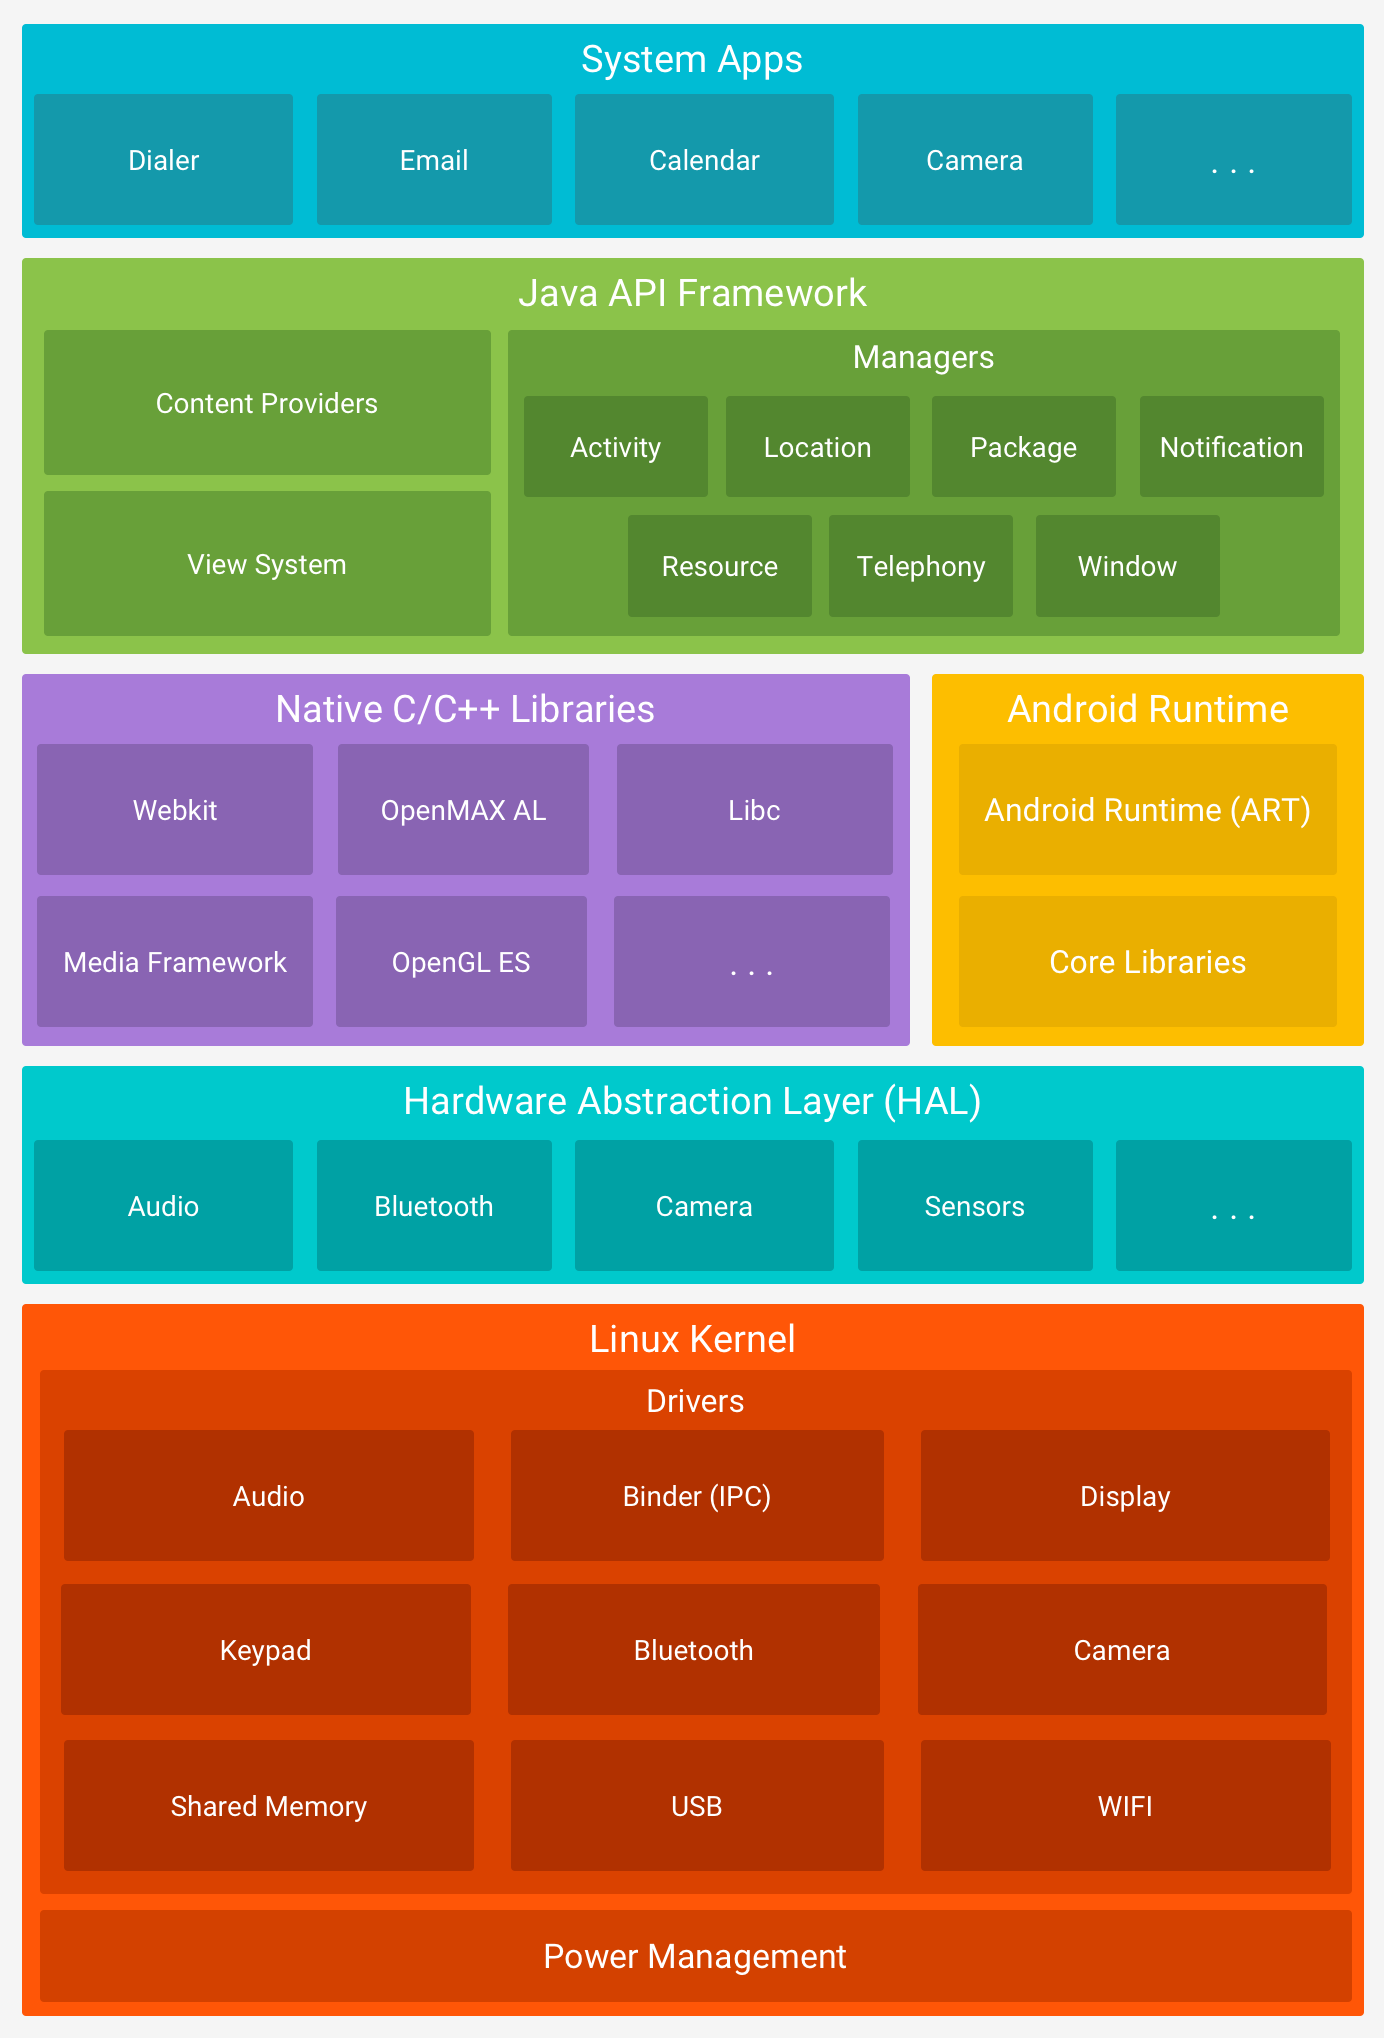
\includegraphics[width=\textwidth]{images/hello/android-stack.png}
	\label{fig:stack}
	\caption{Android is an open source, Linux-based software stack created for a wide array of devices and form factors. The following diagram shows the major components of the Android platform. Figure from \cite{Google2017}}
\end{figure}

\begin{itemize}
	\item \textbf{Linux kernel} The Android Runtime (ART) relies on the Linux kernel for underlying functionalities such as threading and low-level memory management.
	Using a Linux kernel allows Android to take advantage of key security features!
	
	The Linux kernel provides Android with several key security features, including:
	
	\begin{itemize}
		\item A user-based permissions model
	\item Process isolation
	\item Extensible mechanism for secure Inter Proces communication
	\item The ability to remove unnecessary and potentially insecure parts of the kernel
	\end{itemize}
	As a multiuser operating system, a fundamental security objective of the Linux kernel is to isolate user resources from one another. The Linux security philosophy is to protect user resources from one another. Thus, Linux:
	
\begin{itemize}
	\item 	Prevents user A from reading user B's files
	\item Ensures that user A does not exhaust user B's memory
	\item Ensures that user A does not exhaust user B's CPU resources
	\item Ensures that user A does not exhaust user B's devices (e.g. telephony, GPS, Bluetooth)
\end{itemize}
	
	
	
	Moreover, the Linux Kernel  allows device manufacturers to develop hardware drivers for a well-known kernel.
	\item \textbf{Hardware Abstraction Layer (HAL)} The hardware abstraction layer (HAL) provides standard interfaces that expose device hardware capabilities to the higher-level Java API framework. The HAL consists of multiple library modules, each of which implements an interface for a specific type of hardware component, such as the camera or bluetooth module. When a framework API makes a call to access device hardware, the Android system loads the library module for that hardware component.
	\item \textbf{Android Runtime} Each app runs in its own process and with its own instance of the Android Runtime (ART). ART is written to run multiple virtual machines on low-memory devices by executing \textbf{DEX files}, a bytecode format designed specially for Android that's optimized for minimal memory footprint. It uses
	\begin{itemize}
		\item Ahead-of-time (AOT) and just-in-time (JIT) compilation \cite{}
		\item Optimized garbage collection (GC)
	\end{itemize}
	Prior to Android version 5.0 (API level 21), Dalvik was the Android runtime. If your app runs well on ART, then it should work on Dalvik as well, but the reverse may not be true.
	\item \textbf{Native C/C++ Libraries} Many core Android system components and services, such as ART and HAL, are built from native code that require native libraries written in C and C++. 
	\item \textbf{Java API Framework} The entire feature-set of the Android OS is available to you through APIs written in the Java language. These APIs form the building blocks you need to create Android apps by simplifying the reuse of core, modular system components and services.
	\item \textbf{System Apps} Android comes with a set of core apps for email, SMS messaging, calendars, internet browsing, contacts, and more. Apps included with the platform have no special status among the apps the user chooses to install. So a third-party app can become the user's default web browser, SMS messenger, or even the default keyboard (some exceptions apply, such as the system's Settings app).
	
\end{itemize}




\section{Some words on ART}
\subsection{Android Application Development flow}
The way an Android application is built can be seen in figure \ref{fig:develop}. The build process involves many tools and processes that convert your project into an \gls{apk}.

\begin{itemize}
	\item All resource files are combined together by Android Asset Packing Tool (AAPT). Resource files are audio-, video-, image-  and other asset related files. 
	\item Java and Kotlin files are converted into \texttt{.class} files by the compiler. So, the output of the compiler will be \texttt{.class} files, that are the source to put into android. 	\item The \texttt{.class}  files are entered as input to DX tool. Tthis is a tool which will convert \texttt{.class} files to \texttt{.dex} 	 files, which include the bytecode that runs on Android devices, and everything else into compiled resources.
	\item The APK Packager combines the DEX files and compiled resources into a single APK. Before your app can be installed and deployed onto an Android device, however, the APK must be signed.
	\item The APK Packager signs your APK using either the debug or release keystore:
	If you are building a debug version of your app, that is, an app you intend only for testing and profiling, the packager signs your app with the debug keystore. Android Studio automatically configures new projects with a debug keystore.
	If you are building a release version of your app that you intend to release externally, the packager signs your app with the release keystore.
\end{itemize}


\begin{figure}[hb]
	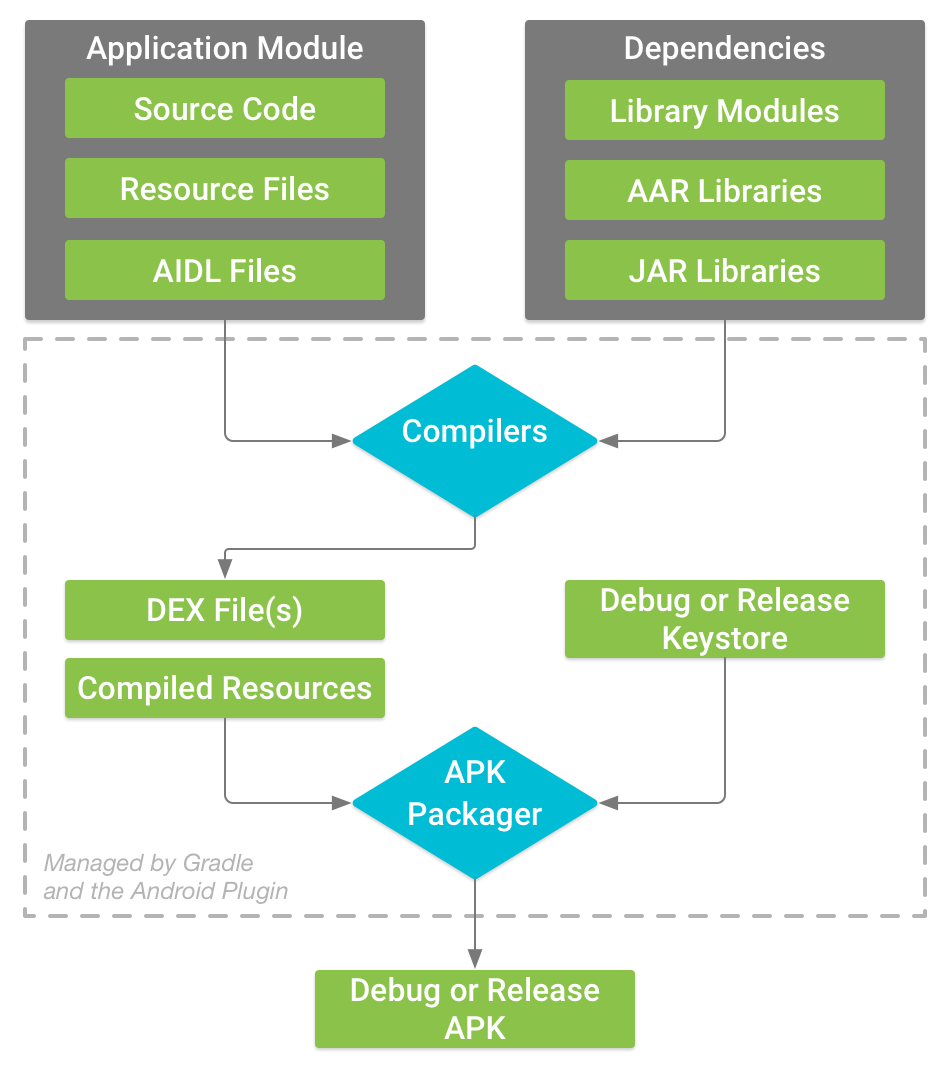
\includegraphics[width=\textwidth]{images/hello/development.png}
	\caption{The flow for building an Android application. Figure from \cite{Developers2018build}}
		\label{fig:develop}
\end{figure}

\subsection{Some words on ART \& Dalvik}
Android runtime (ART) \cite{Android2019} is the managed runtime used by applications and some system services on Android. ART and its predecessor Dalvik were originally created specifically for the Android project. ART as the runtime executes the Dalvik Executable format and Dex bytecode specification.

ART and Dalvik are compatible runtimes running Dex bytecode, so apps developed for Dalvik should work when running with ART. However, some techniques that work on Dalvik do not work on ART. 

The main difference between ART and Dalvik is the compilation method \cite{Vitas2013}. Android apps are deployed in Dalvik bytecode, which is portable, unlike native code. In order to be able to run the app on a device, the code has to be compiled to machine code.

Dalvik is based on JIT (just in time) compilation. It means that each time you run an app, the part of the code required for its execution is going to be translated (compiled) to machine code at that moment. As you progress through the app, additional code is going to be compiled and cached, so that the system can reuse the code while the app is running. Since JIT compiles only a part of the code, it has a smaller memory footprint and uses less physical space on the device.

ART, on the other hand, compiles the intermediate language, Dalvik bytecode, into a system-dependent binary. The whole code of the app will be pre-compiled during install (once), thus removing the lag that we see when we open an app on our device. With no need for JIT compilation, the code should execute much faster.

Except for the potential speed increase, the use of ART can provide an important secondary benefit. As ART runs app machine code directly (native execution), it doesn't hit the CPU as hard as just-in-time code compiling on Dalvik. Less CPU usage results in less battery drain, which is a big plus for portable devices in general.


\section{Package naming \& Versioning}
Android follows normal java package conventions: the package name is used for unique identification for your application. Android uses the package name to determine whether the application has been installed or not. The general naming is:

\begin{center}
	\textbf{com.companyname.applicationname}
\end{center}

\subsection{Minimum SDK}
The Minimum Required SDK is the earliest version of Android that your app supports, indicated using the API level. To support as many devices as possible, you should set this to the lowest version available that allows your app to provide its core feature set. If any feature of your app is possible only on newer versions of Android and it's not critical to the app's core feature set, you can enable the feature only when running on the versions that support it.

\textbf{Generally, it’s a good practice to support about 90\% of the active devices, while targeting your app to the latest version.}

Keep in mind that your dependencies may have their own limitations on minSDKVersions. Hence it is best that your minsSDKVersion is a least the max from the minSDKVersion of your dependencies.

\subsection{Target SDK}
The Target SDK, roughly speaking, is the version of Android you were thinking of when you were writing the code for your app. Usually, you will set this to be the latest shipping Android API level, then change it over time as new versions of Android are released and you decide that you are ready for some of those changes.

\subsection{compileSDKVersion}
compileSdkVersion is your way to tell Gradle what version of the Android SDK to compile your app with. 
It should be emphasized that changing your compileSdkVersion does not change runtime behavior. While new compiler warnings/errors may be present when changing your compileSdkVersion, your compileSdkVersion is not included in your APK: it is purely used at compile time. 

Therefore it is strongly recommended that you always compile with the latest SDK. You’ll get all the benefits of new compilation checks on existing code, avoid newly deprecated APIs, and be ready to use new APIs.

Note that if you use the Support Library, compiling with the latest SDK is a requirement for using the latest Support Library releases. For example, to use the 23.1.1 Support Library, you must have a compileSdkVersion of at least 23 (those first numbers need to match). 

\subsection{Putting it together}
Ideally, your minSDKVersion is the lowest possible, the targetSDKVersion equals the targetSDKVersion and is the latest SDK available.

\section{Gradle}
TODO: stukje rond Gradle


\section{Exercises}
\begin{exercise}
	Download Android Studio, use the latest version. Make all the necessary configurations for your operating system and create a basic project. You can follow the steps explained in \url{https://kotlinlang.org/docs/tutorials/kotlin-android.html}
\end{exercise}

\begin{exercise}
	Review the \texttt{build.gradle} files and try to understand what is written in there. What is happening in these files. What does the \texttt{ext.kotlin\_version} stand for. Is it used somewhere else? Tip: LMGTFY.
\end{exercise}

 \begin{exercise}
 	Our applications will be dependant from several libraries. One of them is ANKO. For some information on ANKO, you can read \cite{Bukros2017}. It is  a library that uses the power of Kotlin to simplify some
 	tasks in Android. We’ll need more parts of Anko later on, but for now it’s enough to
 	add anko-common to your project. 
 \end{exercise}

\begin{exercise}
	In order to test whether everying is working fine, drag a \texttt{TextView} in the layout of a fresh Activity. If you have no Activity, right click your project and create one. We will be covering the Activity later on, for the moment don't worry about it. Try to alter the text at runtime by adding code in the onCreate method. Testing can be done eitther using the emulator or your own machine (if it is connected to your development machine).
\end{exercise}
\chapterimage{images/activities.jpg} % Chapter heading image


\chapter{Activities and Their Lifecycles}
An activity is a single, focused thing that the user can do.
Almost all activities interact with the user, so the Activity class takes care of creating a window for you in which you can place your UI with \texttt{setContentView(View)}. \todo{check if still applicable}
Unlike programming paradigms in which apps are launched with a main() method, the Android system initiates code in an Activity instance by invoking specific callback methods that correspond to specific stages of its lifecycle.

\begin{framed}
	\todo{Aanpassen}
	This chapter has an example application which you can find here \cite{GoogleDevelopers2018}.
	The link contains the steps which youy need to take to build the application.
	The final code can be found on \url{https://github.com/eothein/ActivityProject}	
\end{framed}


\section{Activities}
The Activity class serves as the entry point for an app’s interaction with the user, providing the window in which the app draws its UI.
This window typically fills the screen, but may be smaller than the screen and float on top of other windows.
You implement an activity as a subclass of the Activity class.
Generally, one activity implements one screen in an app.
For instance, one of an app’s activities may implement the Preferences screen, while another activity implements the Compose Email screen.

Most apps contain multiple screens, which means they comprise multiple activities.
Typically, one activity in an app is specified as the main activity, which is the first screen to appear when the user launches the app.
Each activity can then start another one in order to perform different actions.
For example, the main activity in a simple e-mail app may provide the screen that shows an e-mail inbox.
From there, the main activity might launch other activities that provide screens for tasks like writing e-mails and opening individual e-mails.

Although activities work together to form a cohesive user experience in an app, each activity is only loosely bound to the other activities.
It is good practice to keep dependencies between activities to a minimum.
Sometimes activities start up activities belonging to other apps.
For example, a browser app might launch the Share activity of a social-media app.

To use activities in your app, you must register information about them in the app’s manifest, and you must manage activity lifecycles appropriately.

\subsection{One Activity to rule them all}
In the past Android recommended to use one Activity for a single, focuses task for your application.
This resulted in applications with many Activities, all serving a certain purposes.
This architecture had several drawbacks:

\begin{enumerate}
	\item Toolbar configuration and views are handles on different places
	\item You had to rely on the Android Framework to change content
	\item Previous Activities with views could still exist in the stack, which can cause an out-of-memory exception in endless navigation applications
	\item Side menu implementation was difficult.
\end{enumerate}

Android is introducing the Navigation component as a framework for structuring your in-app UI, with a focus on making a single-Activity app the preferred architecture.
Although we are not going to cover the Navigation Component (still in $\alpha$ phase), later in this book we will use the single activity architecture with the corresponding features.
For this chapter however, we will use multiple activities for educational purposes.

\section{The Activity Lifecycle}
As stated before, an activity is a single, focused thing that the user can do.
Almost all activities interact with the user, so the Activity class takes care of creating a window for the UI.

Activities in the system are managed as an activity stack.
When a new activity is started, it is placed on the top of the stack and becomes the running activity.
The previous activity always remains below it in the stack, and will not come to the foreground again until the new activity exits.

The activity lifecycle is demonstrated in figure \ref{fig:lifeCycle1}, which shows the different states and transitions an activity is able to make.
The same model, but maybe a bit more easy to read is shown in figure \ref{fig:lifeCycle2}.
It is up to the reader to see that these figures illustrate the same concept.

As Activities are created and destroyed, they move in and out of the stack \footnote{Activities in the system are managed as an activity stack.
When a new activity is started, it is placed on the top of the stack and becomes the running activity -- the previous activity always remains below it in the stack, and will not come to the foreground again until the new activity exits.} (the "back stack").
As they do so, they transition through four possible states.

\begin{enumerate}
	\item \textbf{Active} - When an Activity is at the top of the stack it is the visible, focused, foreground Activity that is receiving user input.
		Android will attempt to keep it alive at all costs, killing Activities further down the stack as needed, to ensure that it has the resources it needs.
		When another Activity becomes active, this one will be paused.
	\item \textbf{Paused} - In some cases your Activity will be visible but will not have focus; at this point it’s paused.
		This state is reached if a transparent or non-full-screen Activity is active in front.
	\item \textbf{Stopped} - When an Activity isn’t visible, it “stops.” 
		The Activity will remain in memory; however, it is now a candidate for termination when the system requires memory elsewhere.
		When an Activity is in a stopped state, it is important to save data and the current UI state, and to stop any non-critical operations.
	\item \textbf{Inactive} - After an Activity has been killed, and before it’s been launched, it’s inactive.
		Inactive Activities have been removed from the Activity stack and need to be restarted before they can be displayed and used.
\end{enumerate}

\begin{figure}
	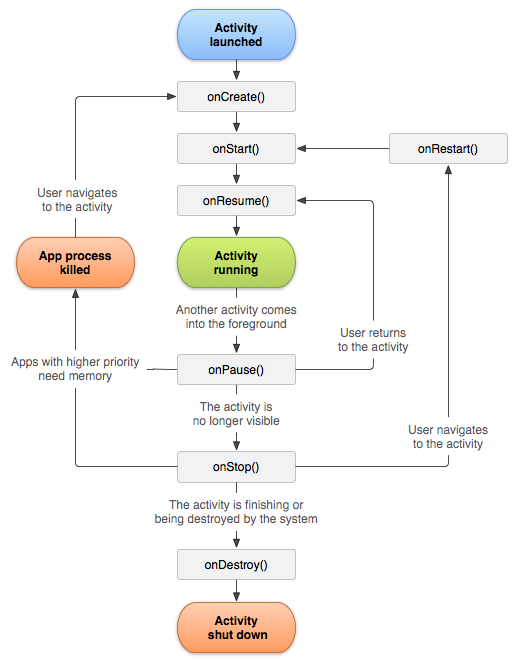
\includegraphics[width=\textwidth]{images/activity/activity_lifecycle1.png}
	\caption{The activity lifecycle, retrieved from \cite{Developers19}}
	\label{fig:lifeCycle1}
\end{figure}

\begin{figure}
	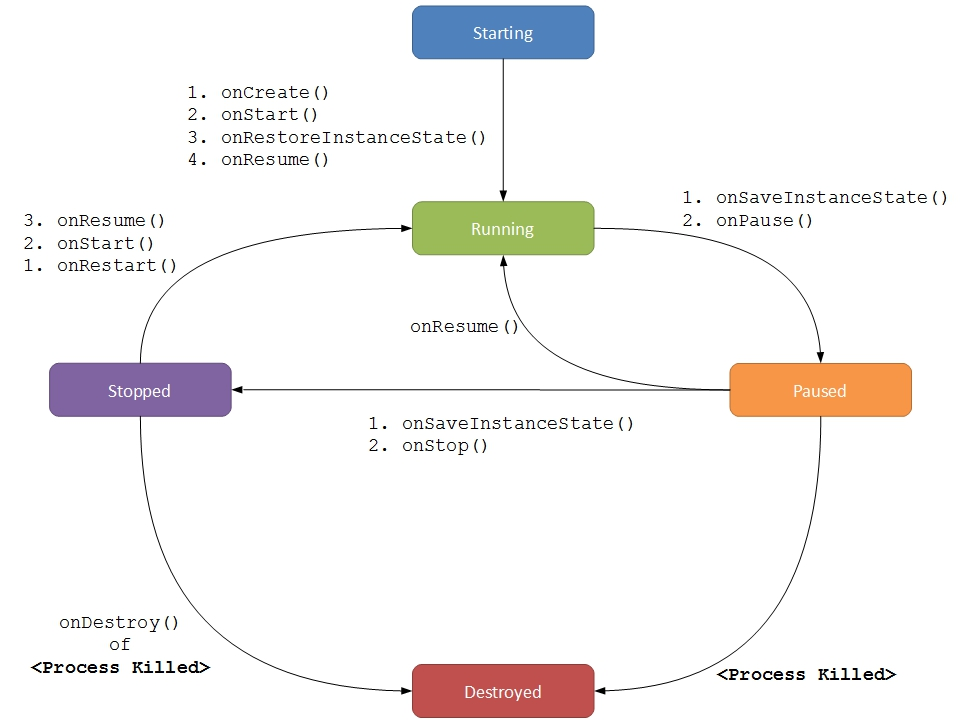
\includegraphics[width=\textwidth]{images/activity/activitylifecycle2.jpg}
		\caption{An even more simplified illustration of the activity lifecycle}
	\label{fig:lifeCycle2}
\end{figure}

For more information regarding the different life cylce callbacks, we refer the reader to \cite{Developers19}.

\subsection{Saving and restoring the state}
There are a few scenarios in which your activity is destroyed due to normal app behavior, such as when the user presses the Back button or your activity signals its own destruction by calling the finish() method.
The system may also destroy the process containing your activity to recover memory if the activity is in the Stopped state and hasn't been used for a long time, or if the foreground activity requires more resources.

When your activity is destroyed because the user presses  ``Back'' or the activity finishes itself, the system's concept of that Activity instance is gone forever because the behavior indicates the activity is no longer needed.
However, if the system destroys the activity due to system constraints (rather than normal app behavior), then although the actual Activity instance is gone, the system remembers that it existed.
When the user navigates back to it, the system creates a new instance of the activity using a set of saved data that describes the state of the activity when it was destroyed.
The saved data that the system uses to restore the previous state is called the \textbf{instance state} and is a collection of key-value pairs stored in a Bundle object.

By default, the system uses the Bundle instance state to save information about each View object in your activity layout (such as the text value entered into an EditText widget).
So, if your activity instance is destroyed and recreated, the state of the layout is restored to its previous state with no code required by you.
However, your activity might have more state information that you'd like to restore, such as member variables that track the user's progress in the activity.

\begin{exercise}
	Start the example application found in \url{https://github.com/eothein/ActivityProject}.
	Remove the id of the editText (\texttt{android:id="@+id/nameEditText"}).
	Fill in your name and turn the device.
	What do you see? What happens when you close the app or press the back button?
\end{exercise}

\subsubsection{Reacting to configuration changes}
Some device configurations can change during runtime (such as screen orientation, keyboard availability, and when the user enables multi-window mode).
When such a change occurs, Android restarts the running Activity ( onDestroy() is called, followed by onCreate()).
The restart behavior is designed to help your application adapt to new configurations by automatically reloading your application with alternative resources that match the new device configuration.

If restarting your activity requires that you recover large sets of data, reestablish a network connection, or perform other intensive operations, then a full restart due to a configuration change might be a slow user experience.
Also, it might not be possible for you to completely restore your activity state with the Bundle the system saves for you with the onSaveInstanceState() callback.
It is not designed to carry large objects (such as bitmaps) and the data within must be serialized and deserialized on the main thread, which can consume a lot of memory and slow down the configuration change.

\subsubsection{Persisting Data Between Launches}
As your activity begins to stop, the system calls the onStop() method so your activity can save state information using a collection of key-value pairs.
The default implementation of this method saves transient information about the state of the activity's view hierarchy, such as the text in an EditText widget or the scroll position of a ListView widget.

When your activity is recreated after it was previously destroyed, you can recover your saved state from the Bundle that the system passes to your activity.
Both the onCreate() and onRestoreInstanceState() callback methods receive the same Bundle that contains the instance state information.

Because the onCreate() method is called whether the system is creating a new instance of your activity or recreating a previous one, you must check whether the state Bundle is null before you attempt to read it.
If it is null, then the system is creating a new instance of the activity, instead of restoring a previous one that was destroyed.

Instead of restoring the state during onCreate() you may choose to implement onRestoreInstanceState(), which the system calls after the onStart() method.
The system calls onRestoreInstanceState() only if there is a saved state to restore, so you do not need to check whether the Bundle is null.

Caution: Always call the superclass implementation of onRestoreInstanceState() so the default implementation can restore the state of the view hierarchy.

Another way of tackling the problem is using Sharedpreferences, which is outlined in the following code example.

\lstinputlisting[firstline=28,lastline=66,language=Kotlin, caption={Persisting Data Between Launches with Shared Preferences}, label=code:KotlinSRPBook]{srccode/activities/MainActivity.kt}



\section{Starting a new activity}
An Intent encapsulates a request send to Android for some activity or other receiver to do something.
If the activity you intend to launch is one of your own, you may find it simplest to create an explicit Intent, naming the component you wish to launch.
For example, from within your activity, you could create an Intent like this:

\begin{lstlisting}
val intent = Intent(this, NextActivity::class.java)
// To pass any data to next activity
intent.putExtra("keyIdentifier", value)
// start your next activity
startActivity(intent)
\end{lstlisting}

This would stipulate that you wanted to launch the NextActivity.
NextActivity would need to have a corresponding <activity> element in your AndroidManifest.xml file.

\section{The Manifest File}
Each Android project includes a manifest file, AndroidManifest.xml, stored in the root of its project hierarchy.
The manifest defines the structure and metadata of your application, its components and its requirements.
In this section we will briefly describe what you can find in the manifest.
The next chapters will take a closer look at it.

\begin{itemize}
	\item It includes nodes for each of the Activities, Services, Content Providers, and Broadcast Receivers that make up your application and, using Intent Filters and Permissions, determines how they interact with each other and with other applications.
	\item The manifest can also specify application metadata (such as its icon, version number, or theme), and additional top-level nodes can specify any required permissions, unit tests, and define hardware, screen, or platform requirements.
	\item The manifest is made up of a root manifest tag with a package attribute set to the project’s package.
		It should also include an xmlns:android attribute that supplies several system attributes used within the file.
	\item Use the versionCode attribute to define the current application version as an integer that increases with each version iteration, and use the versionName attribute to specify a public version that will be displayed to users.
\end{itemize}

\section{Externalizing Resources}
It’s always good practice to keep non-code resources, such as images and string constants, external to your code.
Android supports the externalization of resources, ranging from simple values such as strings and colors to more complex resources such as images (Drawables), animations, themes, and menus.
Perhaps the most powerful externalizable resources are layouts.

By externalizing resources, you make them easier to maintain, update, optimize and manage.
This also lets you easily define alternative resource values for internationalization and to include different resources to support variations in hardware - particularly, screen size and resolution.

\subsection{Strings}
String resources are specified with the string tag and simple markup attributes can be added.
\subsection{Colors}
Use the color tag to define a new color resource.
Specify the color value using a \# symbol followed by the (optional) alpha channel, and then the red, green, and blue values.
\subsection{Drawables}
A drawable resource is a general concept for a graphic that can be drawn to the screen: bitmap and xml descriptions of graphics.
\subsection{Layouts}
Layout resources enable you to decouple your presentation layer from your business logic by designing UI layouts in XML rather than constructing them in code.
You can use layouts to define the UI for any visual component, including Activities, Fragments, and Widgets.
Once defined in XML, the layout must be “inflated” into the user interface.
Within an Activity this is done using setContentView (usually within the onCreate method), whereas Fragment Views are inflated using the inflate method from the Inflator object passed in to the Fragment’s onCreateView handler.
Using layouts to construct your screens in XML is best practice in Android.

\newpage
\section{Exercises}
In this lesson we will build our first working app, using activities, intents and some basic User Interface design.

\begin{exercise}
	In this exercise you create an Activity and count how many times each lifecycle method from the Activity will be called.
	In order to do this you should:
	\begin{enumerate}
		\item Create a new activity with all necessary triggers (all of them)
		\item Log each lifecycle method using a desired logging method.
			Look for some examples online to find the solution that suits you best.
		\item Use a counter variable for each lifecycle method which is incremented with each call of the lifecycle method.
			The user interface should be able to show this counter.
		\item Do this for the first activity.
	\end{enumerate}
	\label{ex:act1}
\end{exercise}

If you are unsure on how to create this functionality, I have one tip: Google!

\begin{exercise}
	Now it is time to create a second activity, with the same functionality as the former.
	We are going to allow the first Activity to start the second activity.
	When you close the second activity, you should see the first activity again.
	You should:
	\begin{enumerate}
		\item Add buttons to both activities (to start the second activity) and one to close the second activity
		\item Implement the method which starts the second activity when the button has been pressed.
		\item Implement the method which stops the second activity and returns to the first activity.
	\end{enumerate}
	\label{ex:act2}
\end{exercise}

At the moment the design of the application is not that important.
Just make sure that the above functionality is implemented.
Don't forget all the good coding standards you have learned during the past years.

\chapter{User Interfaces}

\section{Introduction}
Android gives some key components that can be used to create user interface. All the Android user interface are built using these key components:

\begin{description}
	\item[View] It is the base class for all visual components (control and widgets). All the controls present in an android app are derived
	from this class. A View is an object that draws something on a smartphone screen and enables an user to interact with it.
	\item[Viewgroup] A ViewGroup can contain one or more Views and defines how these Views are placed in the user interface
	(these are used along with Android Layout managers.
	\item[Fragments] This component encapsulates a single piece of UI interface. They are very useful
	when we have to create and optimize our app user interface for multiple devices or multiple screen size.
	\item[Activities] Usually an Android app consists of several activities that exchange data and information. An Activity takes
	care of creating the user interface.
\end{description}

If we analyze in more detail an Android user interface, we can notice that it has an hierarchical structure where at the root there's
a ViewGroup. A ViewGroup behaves like an invisible container where single views are placed following some rules. We
can combine a ViewGroup with another ViewGroup to have more control on how views are located. We have to remember that complex user interfaces require more time to render it. 

\begin{framed}
Therefore, for better performance we should create
simple UIs.  Additionally, a clean interface helps user to have a better experience when using our app.	
\end{framed}


Before we continue we need to define some key concepts:

\begin{description}
	\item[Screen size] It is the physical screen or in other words, the real dimension of our device screen.
	\item[Density] It is the number of pixels in a given area. Usually we consider dot per inch (dpi). This is a measure of the screen
	quality.
	\item[Orientation] This is how the screen is oriented. It can be landscape or portrait.
	\item[Density independent pixel] This is a new pixel unit measure introduced by Android. It is called dp. One dp is equivalent at
	one pixel at a 160dpi screen. We should use dp unit in our measures when creating an UI, at the runtime the system takes care of
	converting it into a real pixel.
\end{description}

From the screen size point of view, Android groups the devices in four areas,small, normal, large and extra large (xlarge),
depending on the actual screen dimension expressed in inches. From the dpi point of view, on the other hand, we can group
devices in: ldpi (low dpi), mdpi (medium dpi), hdpi (high dpi), xhdpi (extra high dpi) and lately xxhdpi. This is important when
we use drawables (i.e bitmaps), because we have to create several images according to the different screen resolution.

There are some best practices regarding the user interface which we would already like to give:

\begin{framed}
	
	
	\begin{enumerate}
		\item Don’t use fixed dimensions expressed in pixel, instead we should use dp.
		\item Provide several layout structures for different screen size, we can do it creating several layout files.
		\item Provide several bitmap with different resolution for different screen resolutions. 
	\end{enumerate}

\end{framed}



\section{Understanding the View}
The View class is the basic class that all the components extend. A View draws something on a piece of screen and it is
responsible to handle events while user interacts with it. Even the generic ViewGroup class extends View. A ViewGroup
is a special View that holds other views and places these views following some rules.


All views have a set of properties: These properties affect the way the view is rendered. There is a set of properties common
to all views, while there are some other properties depending on the type of view.

\begin{description}
	\item[Focus] The system manages the focus on each view and depending on the user input, we can modify and force the focus on a
	specific view.
	\item[Listeners] All views have listeners which are used to handle events when the user interacts with the view. We can register our
	app to listen to specific events that occur on a view.
	\item[Visibility] We can control if a view is visible or not and we can change the view visibility at runtime too.
\end{description}
Two properties that play an important role are \texttt{layout\_width} and \texttt{layout\_height}. These two properties define how large
and how tall should be the view. We can use two predefined values:
\begin{itemize}
	\item \texttt{MATCH\_PARENT} we want our view as big as its parent that holds it
	\item \texttt{WRAP\_CONTENT} we
	specify that our view must be big enough to hold its content.
\end{itemize}
There is another option: using a numeric value. In this case, we specify the exact measure of our view. In this case, the best
practice suggests using dp unit measure so that our view can be adapted to different screen density.


\subsection{You should listen to your View}
Listeners are an important aspect when developing UIs in Android. Generally speaking, when an user interacts with our app
interface, the system “creates” some events. Each view that builds our interface is capable of generating events and providing the means to handle them.

In our Activity there is a method called \texttt{findViewById} that can be used to get the reference to a View defined in our user
interface. Once we have the reference, we can handle the user click:

\begin{android}
b.setOnClickListener(new View.OnClickListener() {
	@Override
	public void onClick(View v) {
		// here we handle the event
	}
});	
\end{android}

\section{Containers and Layoutmanagers}
There are different layout managers which will layout the view it includes. We will not cover them here in detail, but you get a complete overview by checking out the application \texttt{Containers} from \cite{murphymarkl.2017}.




\section{UI consistency}
One of the biggest efforts made by Google was to define a well defined set of rules that helps developers to create appealing user
interfaces. At the same time, these rules help users to navigate through every app in the same way. We call this\textbf{ UI consistency}.
Android, moreover, guarantees to the developers the required flexibility to customize the app look and feel and make it unique.
These rules are known as UI patterns. Patterns are proven solution approaches to well known problems. Thus, having a well
defined UI pattern catalog and knowing when and where apply them, we can create appealing apps that are not only full of
interesting features but they are enjoyable by users and easy to use.

\subsection{The landing activity}
The top level view is the ''landing`` area of our app, so we have to reserve to it a special attention, because this is the first
thing an user sees of our app. There are some specific patterns (see e.g. \cite{Google2017c}) that can be applied when designing this view depending on the type of information we want to show. Some of them are:

\begin{itemize}
	\item \textbf{Fixed tabs} : when we want to give to
	the user an overview of the different views present in our app, so that a user can switch easily between them to show different type of information. See an example here \cite{Tamada2013}
	
	\item \textbf{Spinner}: is used when we want to move directly to a specific view, this is the case of a calendar app when we can use spinner to
	go directly to a specific month.
	
	\begin{xml}
		<Spinner
		android:id="@+id/spinner"
		android:layout_width="fill_parent"
		android:layout_height="wrap_content" />
	\end{xml}
	
	
	\item \textbf{Navigation drawer}: This is a sliding menu, usually at the left side of the
	smartphone screen, that can be opened and closed by the user. This pattern can be used when we have a multiple top level view
	and we want to give to the user a fast access to one of them, or we want to give to the user the freedom to move to one low level
	view directly. For an example see  \cite{Google2017a}
\end{itemize}

\subsection{Detail View}
The detail view is a low level view where a user can interact with data directly. It is used to show data and edit them. In this
kind of view the layout plays an important role to make data well organized and structured. At this level, we can implement
an efficient navigation to improve usability of our app. In fact, we can use swipe view pattern so that user can move between
different detail views. Depending on the type of component we use to show detail information to the user, we can implement
some low level patterns that simplify the user interaction with our app.


\section{Screen and UI performance}
\subsection{Building Views}
For each view in you app, Android goes through three steps to render on the screen:
\begin{itemize}
	\item Measure 
	\item Layout
	\item Draw
\end{itemize}

The measuring starts at the top node and walks the render tree of the layout: measuring the dimensions of each view to be displayed on the screen. Each view will provide dimensions to the parent for positioning. If a parent view discovers an issue in the measurements of the dimensions (or that of its children), it can force every child to remeasure in order to resolve the issue (potentially tripling the measurement time). This is the reason a flat (less nested) view tree is valuable. The deeper the nodes for the tree, the more nested the measurement and the calculation times are lengthened.

See e.g. Instagram! \cite{Kieft2014}


To make sure you don't use to much nested views, you can make use of the Hierarchy Viewer (Component Tree in Android studio): it is a great tool to investigate the construction of your view XML. 

\subsection{Asset reduction}
With a flat design and the number of views reduced, you can reduce the number of objects used in each view. Reusing the objects can be a good strategy here.

\subsection{Overdrawing the screen}
When Android draws the screen, it draws the parent first and then the childer view on top of the parent views. This can result in entire views being drawn on the screen and then these views are entirely cover up by the subsequent views. This is a waist of processor time and should be avoided. 

You can test overdraw using the Debug GPU Overdraw tool in the developer options menu (see \cite{Google2017b}).

 
\newpage
\section{Exercise}

\begin{exercise}
	Pixel art is a form of digital art, created through the use of software, where images are edited on the pixel level. In this exercise you will have to create an application which is able to create such a pixel art drawing. 
	
	Let us have a look at the PixelArt website: \href{https://www.pixilart.com/draw}{PixelArt}. The basic idea of your application is that you make this into an Android application. The following requirements should definitely be fulfilled:
	\begin{enumerate}
		\item Fill in a pixel with a background color by tapping, or sliding over the pixels. There should be a possibility to choose the color for the background.
		\item An extra choice of drawing method: adding text in pixel format, or drawing a circle, or drawing a line or \dots It us up to you which kind of extra drawing technique you implement.
	\end{enumerate}
	Other extra feature will end up in extra credits for this application. 
	
	Off course copy pasting code from existing repositories will end up in a not so pleasant time during the examination.
	
	\label{ex:dotpict}
\end{exercise}
	\begin{figure}[b]
		\centering
	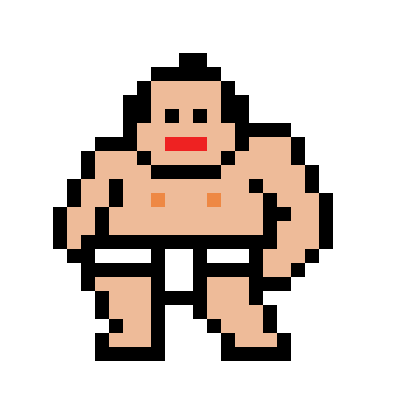
\includegraphics[width=0.4\textwidth]{images/ui/pixelart}
\end{figure}


\chapterimage{images/fragments/fragments.jpg} % Chapter heading image

\chapter{Fragments}
Fragments are an optional layer you can put between your activities and your
widgets, designed to help you reconfigure your activities to support screens both
large (e.g., tablets) and small (e.g., phones). 

If you regard Android as an MVC architecture, fragments and
activities combine to be the controller layer. Fragments serve as a local controller, focused on their set of widgets, populating them from model data, and handling
their events. Activities will serve as more of an orchestration layer, handling cross-
fragment communications (e.g., a click in Fragment A needs to cause a change in what is displayed in Fragment B).

This chapter is built from the following resources: \cite{Point2017, TueDao2017, Guide2017, murphymarkl.2017}.

\section{Design Philopsophy of fragments}
Android introduced fragments in Android 3.0 (API level 11), primarily to support more dynamic and flexible UI designs on large screens, such as tablets. Because a tablet's screen is much larger than that of a handset, there's more room to combine and interchange UI components. Fragments allow such designs without the need for you to manage complex changes to the view hierarchy. By dividing the layout of an activity into fragments, you become able to modify the activity's appearance at runtime and preserve those changes in a back stack that's managed by the activity.

You should design each fragment as a modular and reusable activity component. That is, because each fragment defines its own layout and its own behaviour with its own life cycle callbacks, you can include one fragment in multiple activities, so you should design for reuse and \textbf{avoid directly manipulating one fragment from another fragment}. This is especially important because a modular fragment allows you to change your fragment combinations for different screen sizes.

\section{How to work with activities and fragments}
To explain the use of fragments we will be looking at an example implementation from  \cite{murphymarkl.2017}. You can find the link \href{https://github.com/commonsguy/cw-omnibus/tree/master/Fragments/Static}{here}.

\begin{framed}
	When implementing the exercises for this course you have to use github. Off course you know you do not put every file of your project on the repository. Look how the author of \cite{murphymarkl.2017} have done this on their repository. 
\end{framed}

\subsection{Create a fragment class}

To create a fragment, you must create a subclass of Fragment (or an existing subclass of it). The Fragment class has code that looks a lot like an Activity. It contains callback methods similar to an activity, such as onCreate(), onStart(), onPause(), and onStop().

To provide a layout for a fragment, you must implement the \texttt{onCreateView()} callback method, which the Android system calls when it's time for the fragment to draw its layout. Your implementation of this method must return a \texttt{View} that is the root of your fragment's layout.


\begin{android}
	import android.os.Bundle;
	import android.support.v4.app.Fragment;
	import android.view.LayoutInflater;
	import android.view.ViewGroup;
	
	public class ArticleFragment extends Fragment {
		@Override
		public View onCreateView(LayoutInflater inflater, ViewGroup container,
		Bundle savedInstanceState) {
			// Inflate the layout for this fragment
			return inflater.inflate(R.layout.article_view, container, false);
		}
	}
\end{android}

\subsection{Adding a Fragment (XML)}
To add the fragment, you can
declare the fragment inside the activity's layout file.
	In this case, you can specify layout properties for the fragment as if it were a view. You have to provide the name of the fragment class file.


\begin{xml}
	<LinearLayout xmlns:android="http://schemas.android.com/apk/res/android"
	android:orientation="horizontal"
	android:layout_width="fill_parent"
	android:layout_height="fill_parent">
	
	<fragment android:name="com.example.android.fragments.HeadlinesFragment"
	android:id="@+id/headlines_fragment"
	android:layout_weight="1"
	android:layout_width="0dp"
	android:layout_height="match_parent" />
	
	<fragment android:name="com.example.android.fragments.ArticleFragment"
	android:id="@+id/article_fragment"
	android:layout_weight="2"
	android:layout_width="0dp"
	android:layout_height="match_parent" />
	
	</LinearLayout>
\end{xml}

\begin{android}
	import android.os.Bundle;
	import android.support.v4.app.FragmentActivity;
	
	public class MainActivity extends FragmentActivity {
		@Override
		public void onCreate(Bundle savedInstanceState) {
			super.onCreate(savedInstanceState);
			setContentView(R.layout.news_articles);
		}
	}
\end{android}

\subsection{Adding a Fragment (Programmatically)}
To add the fragment programmatically, you can add the fragment to an existing ViewGroup using FragmentTransaction. 

There are some key concepts which you need to take in mind:
\begin{itemize}
	\item To perform a transaction such as add or remove a fragment, you must use the FragmentManager to create a FragmentTransaction.
	\item You should add the initial fragment(s) to the activity during the activity's onCreate() method.
	\item  Your activity layout must include a container View in which you can insert the fragment. Most of the times this will be an empty FrameLayout.
\end{itemize}

Doing the actual placement, or change or delete:

\begin{android}
	 getSupportFragmentManager().beginTransaction().*
\end{android}

 A simple example can be found \href{https://github.com/commonsguy/cw-omnibus/tree/master/Fragments/Dynamic}{here}.



\subsection{The v4 Support library}
In Android, when using fragments, there are two alternative fragment implementations you can use. One type is the fragment that is provided by the platform version. A platform version corresponds to the version of Android that a user is running. For example, a device running Android 6.0 (SDK Version 23) would be running platform version 23 of the library.
The second type is a support library fragment. When you include a support library, it is added to your project in the same manner as any third-party library. This has two benefits when developing applications for multiple versions of Android.
First, it ensures that you have consistency in your code and functionality across different devices and platform versions. This means that bugs, and fixes, will be more consistent across different versions of Android using these libraries.

Second, when new features are added to the latest version of Android, the Android team will often back-port these features via the support library in order for developers to use on older versions of Android.

\begin{framed}
If you are writing an application that will be targeting multiple versions of Android on multiple devices, you should use support libraries for Fragments. You should also use the support library for any other functionality in your application when available. This is considered a best practice by most senior Android developers and the Core Android team. The only time you might want to use a platform library is if you are, in fact, doing very specialized development for an app that is only targeting one version of Android.
\end{framed}

\section{Fragment Life cycle}
Fragments have lifecycle methods, just like activities do. In fact, they support most
of the same lifecycle methods as activities. You can see an overview in figure \ref{fig:fraglifecycle}.


\begin{figure}
	\centering
	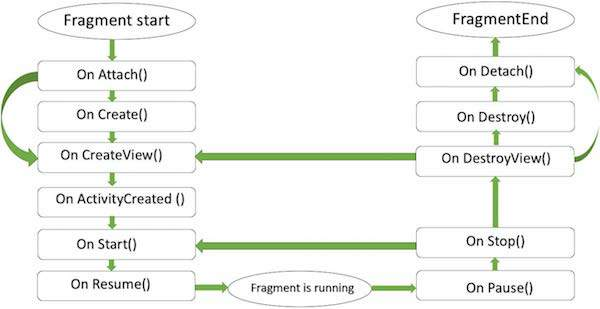
\includegraphics[width=0.8\textwidth]{images/fragments/lifecycle.jpg}
	\caption{Android fragments have their own life cycle very similar to an android activity. Retreived from \cite{Point2017}}
	\label{fig:fraglifecycle}
\end{figure}

The following lifecycle events come into play when you add a fragment:
\begin{description}

\item[onAttach] : When the fragment attaches to its host activity.
\item[onCreate] : When a new fragment instance initializes, which always happens after it attaches to the host — fragments are a bit like viruses.
\item[onCreateView] : When a fragment creates its portion of the view hierarchy, which is added to its activity’s view hierarchy.
\item[onActivityCreated]: When the fragment’s activity has finished its own onCreate event.
\item[onStart] : When the fragment is visible; a fragment starts only after its activity starts and often starts immediately after its activity does.
\item[onResume] : When the fragment is visible and interactable; a fragment resumes only after its activity resumes and often resumes immediately after the activity does.
\item[onPause] : When the fragment is no longer interactable; this occurs when either the fragment is about to be removed or replaced or when the fragment’s activity pauses.
\item[onStop] : When the fragment is no longer visible; this occurs either after the fragment is about to be removed or replaced or when the fragment’s activity stops.
\item[onDestroyView] : When the view and related resources created in onCreateView are removed from the activity’s view hierarchy and destroyed.
\item[onDestroy] : When the fragment does its final clean up.
\item[onDetach] : When the fragment is detached from its activity.
\end{description}
Almost the same rules apply for fragments as do for activities. It is up to the reader to look when each life cycle method is called and when to use it. 

\section{Communication with other Fragments and Activities}

Often you will want one Fragment to communicate with another, for example to change the content based on a user event. All Fragment-to-Fragment communication is done through the associated Activity. 
\begin{framed}
Two Fragments should never communicate directly.
\end{framed}
To allow a Fragment to communicate up to its Activity, you can define an interface in the Fragment class and implement it within the Activity. The Fragment captures the interface implementation during its onAttach() lifecycle method and can then call the Interface methods in order to communicate with the Activity. This way the Fragment can deliver messages to the activity by calling the interface method with a callback instance of the interface defined. 

\section{Communicating from the Activity to the Fragment}
The host activity can deliver messages to a fragment by capturing the Fragment instance with \texttt{findFragmentById()}, then directly call the fragment's public methods.


\section{Exercises}
\begin{exercise}
	Refactor the application you made in exercise \ref{ex:act1} and exercise \ref{ex:act2} in such a way that Fragments are used. You can decide yourself if you prefer dynamic of static fragment setup.
\end{exercise}

\begin{exercise}
	Refactor the application you made in exercise \ref{ex:dotpict}. Your application should:
	\begin{enumerate}
		\item run on large and small devices
		\item landscape and portrait mode
		\item have a layout where the toolbox (tools for drawing your dotpict) is in a fragment, and the drawing itself in another fragment
		\item apply dual pane mode, and single pane mode depending on the orientation or screen size of the device.
	\end{enumerate}
\end{exercise}
\chapterimage{images/intents/intentchapterimage.jpg}

\chapter{Intents and Broadcastreceivers}

\section{Intent}
Intents are objects which you can use for the following actions:


\begin{itemize}
	\item Explicitly start a particular Service or Activity using its class name (already seen in previous lessons)
	\item Implicitly start a particular Service or Activity
	\item Start an Activity or Service to perform an action with (or on) a particular piece of data
	\item Broadcast that an event has occurred
\end{itemize}

The two most important pieces of an Intent are the action and what Android refers
to as the data. If you were to create an Intent combining ACTION\_VIEW with a content Uri of
https://google.com , and pass that Intent to Android via startActivity() ,
Android would know to find and open an activity capable of viewing that resource.


There are other criteria you can place inside an Intent
\begin{description}
	\item[Categories] A string containing additional information about the kind of component that should handle the intent. Any number of category descriptions can be placed in an intent, but most intents do not require a category. Your “main” activity will be in the LAUNCHER category, indicating
	it should show up on the launcher menu.
	\item[A MIME type]  indicating the type of resource you want to operate on.
	\item[Extras] which is a Bundle of other information you want to pass along to
	the receiver with the Intent , that the recipient might want to take advantage
\end{description}

If you specify the target component in your Intent , Android has no
doubt where the Intent is supposed to be routed to — it will launch the named
activity. This might be OK if the target recipient (e.g., the activity to be started) is in your application.

\begin{framed}
		This way of starting components (explicit) is definitely  not recommended for invoking functionality in
		other applications. Component names, by and large, are considered private to the application and are subject to change.
\end{framed}

There are two types of intents.


\subsection{Explicit Intent}
\textbf{An explicit intent} is one that you use to launch a specific app component, such as a particular activity or service in your app. To create an explicit intent, define the component name for the Intent object, all other intent properties are optional.

For example, if you have built a service in your app, named DownloadService, designed to download a file from the web, you can start it with the following code:

\begin{android}
// Executed in an Activity, so 'this' is the Context
// The fileUrl is a string URL, such as "http://www.example.com/image.png"
Intent downloadIntent = new Intent(this, DownloadService.class);
downloadIntent.setData(Uri.parse(fileUrl));
startService(downloadIntent);
\end{android}

\subsection{Implicit intent}
An implicit intent specifies an action that can invoke any app on the device able to perform the action. Using an implicit intent is useful when your app cannot perform the action, but other apps probably can and you'd like the user to pick which app to use.

For example, if you have content that you want the user to share with other people, create an intent with the ACTION\_SEND action and add extras that specify the content to share. When you call startActivity() with that intent, the user can pick an app through which to share the content.

\begin{android}
// Create the text message with a string
Intent sendIntent = new Intent();
sendIntent.setAction(Intent.ACTION_SEND);
sendIntent.putExtra(Intent.EXTRA_TEXT, textMessage);
sendIntent.setType("text/plain");

// Verify that the intent will resolve to an activity
if (sendIntent.resolveActivity(getPackageManager()) != null) {
	startActivity(sendIntent);
}
\end{android}

\begin{framed}
Tt’s good practice to determine if your call will resolve to an Activity before calling startActivity.
\end{framed}

\begin{android}
if (somethingWeird && itDontLookGood) {
	// Create the impliciy Intent to use to start a new Activity.
	Intent intent =
	new Intent(Intent.ACTION_DIAL, Uri.parse(“tel:555-2368”));
	// Check if an Activity exists to perform this action.
	PackageManager pm = getPackageManager();
	ComponentName cn = intent.resolveActivity(pm);
	if (cn == null) {
		// If there is no Activity available to perform the action
		// Check to see if the Google Play Store is available.
		Uri marketUri =
		Uri.parse(“market://search?q=pname:com.myapp.packagename”);
		Intent marketIntent = new Intent(Intent.ACTION_VIEW).setData(marketUri);
		// If the Google Play Store is available, use it to download an application
		// capable of performing the required action. Otherwise log an
		// error.
		if (marketIntent.resolveActivity(pm) != null){
			startActivity(marketIntent);
		}
		else{
			Log.d(TAG, “Market client not available.”);
		}
	}
	else {
		startActivity(intent);
	}
}
\end{android}

\subsection{Allow to start your Activity from another app}

\begin{figure}
	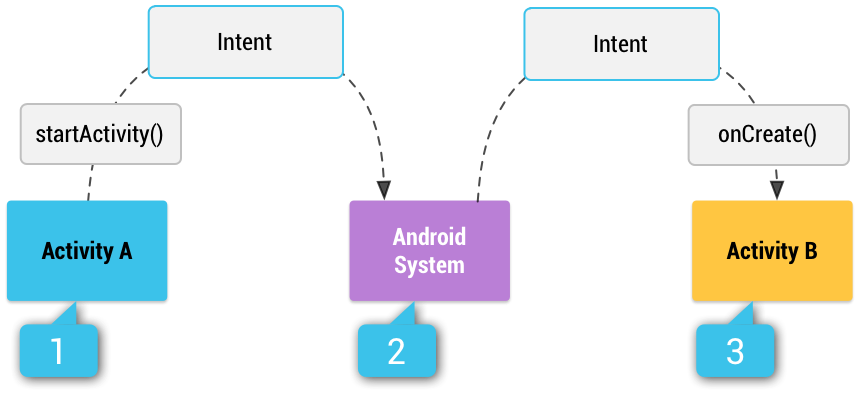
\includegraphics[width=\textwidth]{images/intents/intentresolution.png}
	\caption{Android OS uses filters to pinpoint the set of Activities, Services, and Broadcast receivers that can handle the Intent with help of specified set of action, categories, data scheme associated with an Intent. You will use <intent-filter> element in the manifest file to list down actions, categories and data types associated with any activity, service, or broadcast receiver.}
	\label{fig:intentresolution}
\end{figure}

To allow other apps to start your activity, you need to add an intent-filter element in your manifest file for the corresponding activity element. In order to properly define which intents your activity can handle, each intent filter you add should be as specific as possible in terms of the type of action and data the activity accepts. The system may send a given Intent to an activity if that activity has an intent filter that fulfils the following criteria of the Intent object:

\begin{itemize}
	\item Action : A string naming the action to perform.
	\item Data : A description of the data associated with the intent.
	\item Category: Provides an additional way to characterize the activity handling the intent, usually related to the user gesture or location from which it's started.
\end{itemize}

For example, here's an activity declaration with an intent filter to receive an ACTION\_SEND intent when the data type is text:

\begin{xml}
<activity android:name="ShareActivity">
	<intent-filter>
		<action android:name="android.intent.action.SEND"/>
		<category android:name="android.intent.category.DEFAULT"/>
		<data android:mimeType="text/plain"/>
	</intent-filter>
</activity>
\end{xml}

\section{Broadcastreceiver}
So far, you’ve looked at using Intents to start new application components, but you can also use Intents to broadcast messages anonymously between components via the sendBroadcast() method. As a system-level message-passing mechanism, Intents are capable of sending structured messages across process boundaries. As a result, you can implement Broadcast Receivers to listen for, and respond to, these Broadcast Intents within your applications.

Within your application, construct the Intent you want to broadcast and call sendBroadcast() to send it. Set the action, data, and category of your Intent in a way that lets Broadcast Receivers accurately determine their interest.

\subsection{Receiving a broadcast (without the manifest)}
To receive such a broadcast in an activity (or a fragment), you will need to do four
things.

\begin{enumerate}
	\item you will need to create an instance of your own subclass of
	BroadcastReceiver . The only method you need to (or should) implement is
	onReceive() , which will be passed the Intent that was broadcast, along with a
	Context object that, in this case, you will typically ignore. 
	\item Second, you will need to create an instance of an IntentFilter object, describing
	the sorts of broadcasts you want to receive. Most of these filters are set up to watch
	for a single broadcast Intent action.
	\item You will need to call registerReceiver() , typically from onStart() or onResume() of your
	activity or fragment, supplying your BroadcastReceiver and your IntentFilter .
	\item You will need to call unregisterReceiver() , typically from onStop() or onPause() of your
	activity or fragment, supplying the same BroadcastReceiver instance you provided
	to registerReceiver() .
\end{enumerate}

\subsection{Receiving a broadcast (with the manifest)}
You can also tell Android about broadcasts you wish to receive by adding a
<receiver> element to your manifest, identifying the class that implements your
BroadcastReceiver (via the android:name attribute), plus an <intent-filter> that
describes the broadcast(s) you wish to receive:

\begin{xml}
<receiver android:name=".OnBootReceiver">
	<intent-filter>
		<action android:name="android.intent.action.BOOT_COMPLETED"/>
	</intent-filter>
</receiver
\end{xml}
The good news is that this BroadcastReceiver will be available for broadcasts
occurring at any time. There is no assumption that you have an activity already
running that called registerReceiver() .
The bad news is that the instance of the BroadcastReceiver used by Android to
process a broadcast will live for only so long as it takes to execute the onReceive()
method. At that point, the BroadcastReceiver is discarded. Hence, it is not safe for
a manifest-registered BroadcastReceiver to do anything that needs to run after onReceive()
itself completes, such as forking a thread. After all, Android may well
terminate the process within milliseconds, if there is no other running component
in the process. Moreover, onReceive() is called on the main application thread and may freeze your UI.


\section{Examples}

\begin{example}
	In this example we see an application which is able to convert speech into text. You can find the application here \cite{Buysse18}. This activity contains one button, which will create an special intent launching an Activity which is able to listen to speech, convert it to text and return its results. You will need an actual Android Device to test this. 
	
	The application is also  able to provide the user with a list of extra actions which he is able to perform. The choices are the following:
	\begin{itemize}
		\item pen a web-site with a given url (validate the URL)
		\item Open the contacts
		\item Open the dialer
		\item Search google
	\end{itemize}
Make sure you have a look on the libraries used: Butterknife and Awesomevalidator \cite{Li2016}.
\end{example}


\begin{example}
We will have a good look into the onBoot project from \cite{murphymarkl.2017}: A popular request is to have code get control when the device is powered on. This is
doable but somewhat dangerous, in that too many on-boot requests slow down the
device startup and may make things sluggish for the user.
\end{example}

\begin{example}
	There is an ACTION\_BATTERY\_CHANGED Intent that gets broadcast as the battery
	status changes, both in terms of charge (e.g., 80\% charged) and charging (e.g., the
	device is now plugged into AC power). You simply need to register to receive this
	Intent when it is broadcast, then take appropriate steps. See the full code in \cite{murphymarkl.2017}.
\end{example}

\pagebreak

\section{Exercise}
\begin{exercise}
	It is time to modify our Dotpict application even further. Make sure your application is able to open the camera application for taking pictures. When a picture has been taken, your application should be able to process the photo and convert it into a pixelated version (using the views or strategy you have already provided in the previous exercises).
\end{exercise}



\chapterimage{images/recycler/recycling.jpg}
\chapter{Recyclerview}
In 2014, Google released RecyclerView , via the Android Support package.
Developers can add the recyclerview-v7 to their projects and use RecyclerView. In this chapter, we will review RecyclerView from the ground up, starting with basic
operation.

Before you are able to use the recylceview,  open build.gradle (app) and add the dependencies needed.

\begin{xml}
    compile 'com.android.support:recyclerview-v7:+'
	compile 'com.android.support:cardview-v7:+'
\end{xml}

\section{What is a recyclerview}
The RecyclerView is a new ViewGroup that is prepared to render any adapter-based view. It is supposed to be the successor of ListView and GridView, and it can be found in the latest support-v7 version. One of the reasons is that RecyclerView has a more extensible framework, especially since it provides the ability to implement both horizontal and vertical layouts. Use the RecyclerView widget when you have data collections whose elements change at runtime based on user action or network events.

To use a recyclerview, you will need the following things:
\begin{enumerate}
	\item RecyclerView.Adapter - To handle the data collection and bind it to the view
	\item A layout file defining the row layout in the recyclerview. Just a note here: when you create the item layout of the RecyclerView don’t forget to add the following lines in the ViewGroup container of the layout. This lines of code will add the ripple effect to the RecyclerView elements.
	\begin{enumerate}
		\item  android:clickable="true"
		\item android:focusable="true"
		\item android:foreground="?android:attr/selectableItemBackground"
	\end{enumerate}
	\item LayoutManager - Helps positioning the items
	\item ItemAnimator - Helps with animating the items for common operations such as Addition or Removal of item
\end{enumerate}


\section{Components and Workflow}

\begin{figure}
	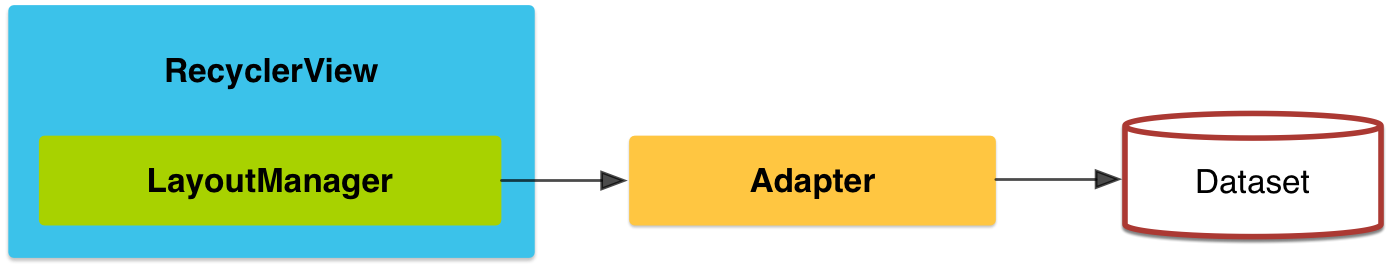
\includegraphics[width=\textwidth]{images/recycler/components.png}
	\caption{ RecyclerView is a major enhancement over ListView. It contains many new features like ViewHolder, ItemDecorator, LayoutManager, and SmoothScroller. But one thing that certainly gives it an edge over the ListView is; the ability to have animations while adding or removing an item. }
	\label{fig:recyclercomponents}
\end{figure}


\subsection{RecyclerView.Adapter}
RecyclerView uses an adapter to help convert our model data
into visual representations. A RecyclerView.Adapter  uses a generic to identify a ViewHolder that will be responsible for doing the work to actually tie
model data to row widgets.

RecyclerView.Adapter has three abstract methods that need to be implemented.

\begin{enumerate}
	\item getItemCount() , which fills the same role as does getCount() indicating how many items there will be in the RecyclerView
	\item onCreateViewHolder()  needs to create, configure,
	a ViewHolder for a particular row of our list. It is passed two parameters:
	\begin{enumerate}
		\item a ViewGroup that will hold the views managed by the holder, mostly for use
		with layout inflation, and
		\item an int that is the particular view type we are using, for cases where we have
		multiple view types
	\end{enumerate}
	\item onBindViewHolder()
	is responsible for updating a ViewHolder based upon the
	model data for a certain position .
\end{enumerate}

\subsection{ViewHolder}
The RecyclerView.ViewHolder is responsible for binding data as needed from our
model into the widgets for a row in our list. However, other than needing to use the base class of RecyclerView.ViewHolder ,
there is no other particular protocol that is mandated between the adapter and the
view holder. You can invent your own API.

This solution avoids all the findViewById() method calls in the adapter to find the views to be filled with data.

\subsection{LayoutManagers}
After adding a recyclerview to the activity, the first thing we do is call setLayoutManager() ,
which will associate a RecyclerView.LayoutManager with our RecyclerView, for example a LinearLayoutManager. RecyclerView
knows absolutely nothing about how to lay out its children. That work is delegated
to a RecyclerView.LayoutManager , so that different approaches can be plugged in as
needed.

There are three concrete subclasses of the abstract RecyclerView.LayoutManager
base class that ship with recyclerview-v7 :
\begin{enumerate}
	\item LinearLayoutManager , which implements a vertically-scrolling list
	\item GridLayoutManager ,
	which implements a two-dimensional vertically-
	scrolling list
	\item StaggeredGridLayoutManager , which implements a “staggered grid”, which
	has columns of cells like a GridView , but where the cells do not have to all
	have the same size.
\end{enumerate}


\subsection{ItemAnimator}
RecyclerView.ItemAnimator is a class that defines the animations performed on items and will animate ViewGroup changes such as add/delete/select notified to the adapter. DefaultItemAnimator is a basic animation available by default with the RecyclerView.

To customize the DefaultItemAnimator add an item animator to the RecyclerView. 


\subsection{Responding to Clicks}
Even though displaying elements in RecyclerView is better, in terms of performance, than its predecessors, ListView and GridView, it is not simple to add a clicklistener. 

To overcome this problem create an Interface

\begin{android}
public interface RecyclerViewItemClickListener {
	public void onClick(View view, int position);
	
	public void onLongClick(View view, int position);
}
\end{android}
To detect the item of the RecyclerView which is clicked we need a helper class.

\begin{android}
public class CustomRVItemTouchListener implements RecyclerView.OnItemTouchListener {
	
	//GestureDetector to intercept touch events
	GestureDetector gestureDetector;
	private RecyclerViewItemClickListener clickListener;
	
	public CustomRVItemTouchListener(Context context, final RecyclerView recyclerView, final RecyclerViewItemClickListener clickListener) {
		this.clickListener = clickListener;
		gestureDetector = new GestureDetector(context, new GestureDetector.SimpleOnGestureListener() {
			
			@Override
			public boolean onSingleTapUp(MotionEvent e) {
				return true;
			}
			
			@Override
			public void onLongPress(MotionEvent e) {
				//find the long pressed view
				View child = recyclerView.findChildViewUnder(e.getX(), e.getY());
				if (child != null && clickListener != null) {
					clickListener.onLongClick(child, recyclerView.getChildLayoutPosition(child));
				}
			}
		});
	}
	
	@Override
	public boolean onInterceptTouchEvent(RecyclerView recyclerView, MotionEvent e) {
		
		View child = recyclerView.findChildViewUnder(e.getX(), e.getY());
		if (child != null && clickListener != null && gestureDetector.onTouchEvent(e)) {
			clickListener.onClick(child, recyclerView.getChildLayoutPosition(child));
		}
		return false;
	}
	
	@Override
	public void onTouchEvent(RecyclerView rv, MotionEvent e) {
		
	}
	
	@Override
	public void onRequestDisallowInterceptTouchEvent(boolean disallowIntercept) {
		
	}
}
\end{android}

Basically what this class does is, detect the RecyclerView element under the (X, Y) position where the screen was clicked. This class is helpful for both click types created by the interface.


\section{CardView}
Cards are a popular visual metaphor in mobile development. Dividing content collections (or aspects of a larger piece of content) into cards makes it clearer how you can reorganize that content to fit various screen sizes and orientations. In some cases, you might have a single column of cards, while in other cases, you have cards
arranged more laterally.

In 2014, Google released cardview-v7 , another library in the Android Support
package, that offers a CardView . CardView is a simple subclass of FrameLayout ,
designed to provide a card UI, consisting of a rounded rectangle and a drop shadow.
In particular, CardView will use Android 5.0’s default drop shadows based on widget
elevation, while offering emulated drop shadows on earlier Android releases. This
way, you can get a reasonably consistent look going back to API Level 7.
To use this, you will have to add the cardview-v7 library to your app project.
Android Studio users can just add a dependency on the cardview-v7 artifact in the
Android Support repository

\section{Example}

\begin{example}
	In the repository found here \cite{Buysse2017}, we find an example demonstrating the principles explained above. Moreover, it makes use of a Fragment with a Recyclerview. It uses Butterknife as already demonstrated in previous example. For loading the images it makes use of the Picasso library (see \cite{Square2017}). 
\end{example}

\newpage
\section{Exercise}
\begin{exercise}
	Interview some of your classmates: ask their traits which describe them best. After the interview, make a nice picture (after asking permission of course).
	
	With this information in place, you should implement the following game: Guess who! If you don't know the game, see \cite{WikiHow2017}.
	
	The game should be able to be played in portrait and in landscape mode.
	Portrait mode should only contain a recyclerview with a small description of the student. The student should be able to be swiped out (i.e. he does not meet de traits). Pressing a student should show a new fragment with the student's description.
	Landscape mode should contain the list plus the description of the student. Swiping again deletes the student and the corresponding detailfragment.
	You should be able to restart the game.
	Make sure you apply the give best practices and try to animate as much as possible!
\end{exercise}


\chapterimage{images/persistency/persistence.jpg}

\chapter{Persistence}
In this Chapter we will review some of the persistence methods use in Android. We will have a look into saving a small portion of data and a more structured (relational) type of data.

\section{Shared preferences}
If you have a relatively small collection of key-values that you'd like to save, you should use the SharedPreferences APIs. A SharedPreferences object points to a file containing key-value pairs and provides simple methods to read and write them. Each SharedPreferences file is managed by the framework and can be private or shared.

\subsection{Creating shared preferences}
Using the SharedPreferences class, you can create named maps of name/value pairs that can be persisted across sessions and shared among application components running within the same application sandbox. To create or modify a Shared Preference, call getSharedPreferences on the current Context, passing in the name of the Shared Preference to change.

Shared Preferences are stored within the application’s sandbox, so they can be shared between an application’s components but aren’t available to other applications. To modify a Shared Preference, use the SharedPreferences.Editor class. Get the Editor object by calling edit on the Shared Preferences object you want to change.

To save edits, call apply on the Editor object to save the changes asynchronously.
\begin{android}
SharedPreferences mySharedPreferences = getSharedPreferences(MY_PREFS, 
Activity.MODE_PRIVATE);
SharedPreferences.Editor editor = mySharedPreferences.edit();
// Store new primitive types in the shared preferences object.
editor.putBoolean(“isTrue”, true);
editor.putFloat(“lastFloat”, 1f);
editor.putInt(“wholeNumber”, 2);
editor.putLong(“aNumber”, 3l);
editor.putString(“textEntryValue”, “Not Empty”);
editor.apply();
\end{android}


\subsection{Retrieving shared preferences}
Accessing Shared Preferences, like editing and saving them, is done using the getSharedPreferences method. Use the type-safe get methods to extract saved values. Each getter takes a key and a default value (used when no value has yet been saved for that key.)

\begin{android}
// Retrieve the saved values.
boolean isTrue = mySharedPreferences.getBoolean(“isTrue”, false);
float lastFloat = mySharedPreferences.getFloat(“lastFloat”, 0f);
int wholeNumber = mySharedPreferences.getInt(“wholeNumber”, 1);
long aNumber = mySharedPreferences.getLong(“aNumber”, 0);
String stringPreference =
mySharedPreferences.getString(“textEntryValue”, “”);
\end{android}

\section{SQLLite}
Using SQLite you can create fully encapsulated relational databases for your applications. Use them to store and manage complex, structured application data. Android databases are stored in the \texttt{/data/data/<package\_name>/databases} folder on your device (or emulator). All databases are private, accessible only by the application that created them.

\subsection{Define your Schema}
One of the main principles of SQL databases is the schema: a formal declaration of how the database is organized. The schema is reflected in the SQL statements that you use to create your database. You may find it helpful to create a companion class, known as a contract class, which explicitly specifies the layout of your schema in a systematic and self-documenting way.

A contract class is a container for constants that define names for URIs, tables, and columns. The contract class allows you to use the same constants across all the other classes in the same package. This lets you change a column name in one place and have it propagate throughout your code.

A good way to organize a contract class is to put definitions that are global to your whole database in the root level of the class. Then create an inner class for each table that enumerates its columns.

Note: By implementing the BaseColumns interface, your inner class can inherit a primary key field called \_ID that some Android classes such as cursor adaptors will expect it to have. It's not required, but this can help your database work harmoniously with the Android framework.


\subsection{Introducing the SQLiteOpenHelper}
SQLiteOpenHelper is an abstract class used to implement the best practice pattern for creating, opening, and upgrading databases. By implementing an SQLite Open Helper, you hide the logic used to decide if a database needs to be created or upgraded before it’s opened, as well as ensure that each operation is completed efficiently. It’s good practice to defer creating and opening databases until they’re needed. The SQLiteOpen Helper caches database instances after they’ve been successfully opened, so you can make requests to open the database immediately prior to performing a query or transaction. For the same reason, there is no need to close the database manually unless you no longer need to use it again.

\begin{framed}
	Database operations, especially opening or creating databases, can be time consuming. To ensure this doesn’t impact the user experience, make all database transactions asynchronous. Make sure you use the same connection when writing and reading to the database (where locking is implemented).
\end{framed}

To access a database using the SQLite Open Helper, call getWritableDatabase or getReadableDatabase to open and obtain a writable or read-only instance of the underlying database, respectively.

You need to override the following methods to create and update your database.
\begin{enumerate}
	\item onCreate() - is called by the framework, if the database is accessed but not yet created.
	\item onUpgrade() - called, if the database version is increased in your application code. This method allows you to update an existing database schema or to drop the existing database and recreate it via the onCreate() method.
	\item  onOpen() - This method is called after the database connection has been configured and after the database schema has been created, upgraded or downgraded as necessary.
\end{enumerate}

\begin{framed}
It is good practice to create a separate class per table. This class defines static onCreate() and onUpgrade() methods. These methods are called in the corresponding methods of SQLiteOpenHelper. This way your implementation of SQLiteOpenHelper stays readable, even if you have several tables.
\end{framed}

\subsubsection{Some considerations}
You should keep the following Android-specific considerations in mind when designing your database.
\begin{enumerate}
	\item Files (such as bitmaps or audio fi les) are not usually stored within database tables. Use a string to store a path to the fi le, preferably a fully qualifi ed URI.
	\item Although not strictly required, it’s strongly recommended that all tables include an auto-increment key field as a unique index field for each row. If you plan to share your table using a Content Provider, a unique ID field is required.
\end{enumerate}

\subsection{Query a database}
Each database query is returned as a \texttt{Cursor}. This lets Android manage resources more efficiently by retrieving and releasing row and column values on demand. To execute a query on a Database object, use the query method with the necessary parameters.

\subsubsection{Cursor}
A query returns a Cursor object. A Cursor represents the result of a query and basically points to one row of the query result. This way Android can buffer the query results efficiently; as it does not have to load all data into memory.

To extract values from a Cursor, first use the \texttt{moveTo<location>} method to position the cursor at the correct row of the result Cursor, and then use the type-safe \texttt{get<type>} methods (passing in a column index) to return the value stored at the current row for the specified column. To find the column index of a particular column within a result Cursor, use its \texttt{getColumnIndexOrThrow} and \texttt{getColumnIndex()} methods. As an overview:

To get the number of elements of the resulting query use the \texttt{getCount()} method.
To move between individual data rows, you can use the \texttt{moveToFirst()} and \texttt{moveToNext()} methods. The \texttt{isAfterLast()} method allows to check if the end of the query result has been reached.
Cursor provides typed get*() methods, e.g. \texttt{getLong(columnIndex)}, \texttt{getString(columnIndex)} to access the column data for the current position of the result. The "columnIndex" is the number of the column you are accessing.
Cursor also provides the \texttt{getColumnIndexOrThrow(String)} method which allows to get the column index for a column name of the table.
When you have finished using your result Cursor, it’s important to close it to avoid memory leaks and reduce your application’s resource load

\subsection{Insert into a database}
To create a new row, construct a ContentValues object and use its put methods to add name/value pairs representing each column name and its associated value. Insert the new row by passing the Content Values into the insert method called on the target database — along with the table name.

\subsection{Updating a row}
When you need to modify a subset of your database values, use the update() method.

Updating the table combines the content values syntax of insert() with the where syntax of delete().

\subsection{Deleting a row}
To delete rows from a table, you need to provide selection criteria that identify the rows. The database API provides a mechanism for creating selection criteria that protects against SQL injection. The mechanism divides the selection specification into a selection clause and selection arguments. The clause defines the columns to look at, and also allows you to combine column tests. The arguments are values to test against that are bound into the clause. Because the result isn't handled the same as a regular SQL statement, it is immune to SQL injection.

\subsubsection{SQL Injection}
Just like web applications, Android applications may use untrusted input to construct SQL queries and do so in a way that's exploitable (see \cite{Makan2013}). The most common case is when applications do not sanitize input for any SQL and do not limit access to content providers.

Why would you want to stop a SQL-injection attack? Well, let's say you're in the classic situation of trying to authorize users by comparing a username supplied by querying a database for it. The code would look similar to the following:

\begin{android}
public boolean isValidUser(){ 
	u_username = EditText( some user value );
	u_password = EditText( some user value );
	//some un-important code here...
	String query = "select * from users_table 
	where username = '" +  u_username + "' and password = '" + 
	u_password
	+"'";
	SQLiteDatabase db
	//some un-important code here...
	Cursor c = db.rawQuery( p_query, null );
	return c.getCount() != 0;
}
\end{android}
What's the problem in the previous code? Well, what happens when the user supplies a password '' or '1'='1'? The query being passed to the database then looks like the following:

\begin{android}
select * from users_table where username = '" +  
u_username
+ "' and password = '' 
or '1'='1'
"
\end{android}

The preceding bold characters indicate the part that was supplied by the user; this query forms what's known in Boolean algebra as a logical tautology; meaning no matter what table or data the query is targeted at, it will always be set to true, which means that all the rows in the database will meet the selection criteria. This then means that all the rows in \texttt{users\_table} will be returned and as result, even if a nonvalid password ' or '1'=' is supplied, the c.getCount() call will always return a nonzero count, leading to an authentication bypass!

The best way to make sure adversaries will not be able to inject unsolicited SQL syntax into your queries is to avoid using SQLiteDatabase.rawQuery() instead opting for a parameterized statement. Using a compiled statement, such as SQLiteStatement, offers both binding and escaping of arguments to defend against SQL-injection attacks. Also, there is a performance benefit due to the fact the database does not need to parse the statement for each execution. An alternative to SQLiteStatement is to use the query, insert, update, and delete methods on SQLiteDatabase as they offer parameterized statements via their use of string arrays.

When we describe parameterized statement, we are describing an SQL statement with a question mark where values will be inserted or binded. Here's an example of parameterized SQL insert statement:

\section{Working assynchronoysly with SQLLite}
\subsection{Loaders}
Loaders are  simple, self-contained objects that (1) load data on a separate thread, and (2) monitor the underlying data source for updates, re-querying when changes are detected. The Loader API lets you load data from a content provider or other data source for display in an Activity or Fragment.
\begin{itemize}
	\item If you fetch the data directly in the activity or fragment, your users will suffer from lack of responsiveness due to performing potentially slow queries from the UI thread.
	\item If you fetch the data from another thread, perhaps with AsyncTask, then you're responsible for managing both the thread and the UI thread through various activity or fragment lifecycle events, such as onDestroy() and configurations changes. Using Loaders this is not necessary.
\end{itemize}

\subsection{Loadersmanager}
The LoaderManager is responsible for managing one or more Loaders associated with an Activity or Fragment. Each Activity and each Fragment has exactly one LoaderManager instance that is in charge of starting, stopping, retaining, restarting, and destroying its Loaders. These events are sometimes initiated directly by the client, by calling initLoader(), restartLoader(), or destroyLoader(). Just as often, however, these events are triggered by major Activity/Fragment lifecycle events. For example, when an Activity is destroyed, the Activity instructs its LoaderManager to destroy and close its Loaders (as well as any resources associated with them, such as a Cursor).

The LoaderManager does not know how data is loaded, nor does it need to. Rather, the LoaderManager instructs its Loaders when to start/stop/reset their load, retaining their state across configuration changes and providing a simple interface for delivering results back to the client. 

The LoaderManager makes your life easy. It initializes, manages, and destroys Loaders for you, reducing both coding complexity and subtle lifecycle-related bugs in your Activitys and Fragments. Further, interacting with the LoaderManager involves implementing three simple callback methods.

\subsection{LoaderManager.LoaderCallbacks<D>}
The LoaderManager.LoaderCallbacks<D> interface is a simple contract that the LoaderManager uses to report data back to the client. Each Loader gets its own callback object that the LoaderManager will interact with. This callback object fills in the gaps of the abstract LoaderManager implementation, telling it how to instantiate the Loader (onCreateLoader) and providing instructions when its load is complete/reset (onLoadFinished and onLoadReset, respectively). Most often you will implement the callbacks as part of the component itself, by having your Activity or Fragment implement the LoaderManager.LoaderCallbacks<D> interface:

\begin{android}
public class SampleActivity extends Activity implements LoaderManager.LoaderCallbacks<D> {
	
	public Loader<D> onCreateLoader(int id, Bundle args) { ... }
	
	public void onLoadFinished(Loader<D> loader, D data) { ... }
	
	public void onLoaderReset(Loader<D> loader) { ... }
	
	/* ... */
}	
\end{android}

Once instantiated, the client passes the callbacks object  as the third argument to the LoaderManager’s initLoader method, and will be bound to the Loader as soon as it is created.

Overall, implementing the callbacks is straightforward. Each callback method serves a specific purpose that makes interacting with the LoaderManager easy:

\begin{enumerate}
	\item onCreateLoader is a factory method that simply returns a new Loader. The LoaderManager will call this method when it first creates the Loader.
	
	\item onLoadFinished is called automatically when a Loader has finished its load. This method is typically where the client will update the application’s UI with the loaded data. The client may (and should) assume that new data will be returned to this method each time new data is made available. Remember that it is the Loader’s job to monitor the data source and to perform the actual asynchronous loads. The LoaderManager will receive these loads once they have completed, and then pass the result to the callback object’s onLoadFinished method for the client (i.e. the Activity/Fragment) to use.
	
	\item onLoadReset is called when the Loader’s data is about to be reset. This method gives you the opportunity to remove any references to old data that may no longer be available.
\end{enumerate}

\section{Content Providers}
ContentProviders  provide an interface for publishing data that will be consumed using a ContentResolver. They allow you to decouple the application components that consume data from their underlying data sources, providing a generic mechanism through which applications can share their data or consume data provided by others.

You will also need to override the onCreate handler to initialize the underlying data source, as well as the query, update, delete, insert, and getType methods to implement the interface used by the Content Resolver to interact with the data.

\begin{framed}
	Like the database contract class described in the previous section, it’s good practice to include static ContentProvider constants — particularly column names and the Content Provider authority — that will be required for transacting with, and querying, the database.
\end{framed}

\subsection{Registering Content Providers}
Like Activities and Services, Content Providers must be registered in your application manifest before the Content Resolver can discover them. This is done using a provider tag that includes a name attribute describing the Provider’s class name and an authorities tag.

Use the authorities tag to define the base URI of the Provider’s authority. A Content Provider’s authority is used by the Content Resolver as an address and used to find the data source you want to interact with.

\begin{framed}
Each Content Provider authority must be unique, so it’s good practice to base the URI path on your package name e.g., \texttt{com.<CompanyName>.provider.<ApplicationName>}
\end{framed}

\begin{xml}
<provider
android:authorities="com.hogent.provider.testapplicatie"
android:name=".contentprovider.TestContentProvider" >
</provider>
\end{xml}

Until Android version 4.2 a content provider is by default available to other Android applications. As of Android 4.2 a content provider must be explicitly exported. To set the visibility of your content provider use the android:exported=false|true parameter in the declaration of your content provider in the AndroidManifest.xml file.

You can use a UirMatcher to help you with the Uri matching.

\subsection{Creating the ContentProvider's data source}
To initialize the data source you plan to access through the Content Provider, override the onCreate method. This is typically handled using an SQLite Open Helper implementation, of the type described in the previous section, allowing you to effectively defer creating and opening the database until it’s required.

To support queries with your Content Provider, you must implement the query and getType methods. Content Resolvers use these methods to access the underlying data, without knowing its structure or implementation. These methods enable applications to share data across application boundaries without having to publish a specific interface for each data source. The most common scenario is to use a ContentProvider to provide access to an SQLite database, but within these methods you can access any source of data (including files, application instance variables or even the network).

Having implemented queries, you must also specify a MIME type to identify the data returned. Override the getType method to return a string that uniquely describes your data type.

To expose delete, insert, and update transactions on your Content Provider, implement the corresponding delete, insert, and update methods.

When performing transactions that modify the dataset, it’s good practice to call the Content Resolver’s \texttt{notifyChange} method. This will notify any Content Observers, registered for a given Cursor using the Cursor.registerContentObserver method, that the underlying table (or a particular row) has been removed, added, or updated.

\subsection{ContentResolver}
Each application includes a ContentResolver instance, accessible using the getContentResolver method. When Content Providers are used to expose data, Content Resolvers are the corresponding class used to query and perform transactions on those Content Providers. Whereas Content Providers provide an abstraction from the underlying data, Content Resolvers provide an abstraction from the Content Provider being queried or transacted. The Content Resolver includes query and transaction methods corresponding to those defi ned within your Content Providers. The Content Resolver does not need to know the implementation of the Content Providers it is interacting with — each query and transaction method simply accepts a URI that specifi es the Content Provider to interact with.

To retrieve data from a provider, follow these basic steps:

\begin{enumerate}
	\item Request the read access permission for the provider.
	\item Define the code that sends a query to the provider.
\end{enumerate}


To retrieve data from a provider, your application needs "read access permission" for the provider. You can't request this permission at run-time; instead, you have to specify that you need this permission in your manifest, using the <uses-permission>; element and the exact permission name defined by the provider. When you specify this element in your manifest, you are in effect "requesting" this permission for your application. When users install your application, they implicitly grant this request.

Using the query method on the ContentResolver object, pass in the following:

\begin{enumerate}
	\item A URI to the Content Provider you want to query.
	\item A projection that lists the columns you want to include in the result set.
	\item A where clause that defi nes the rows to be returned. You can include ? wildcards that will be replaced by the values passed into the selection argument parameter.
	\item An array of selection argument strings that will replace the ? wildcards in the where clause.
	\item A string that describes the order of the returned rows.
\end{enumerate}

\subsection{Querying for Content Asynchronously Using the CursorLoader}
To use a Cursor Loader, create a new LoaderManager.LoaderCallbacks implementation. Loader Callbacks are implemented using generics, so you should specify the explicit type being loaded, in this case Cursors, when implementing your own.

\begin{android}
LoaderManager.LoaderCallbacks<Cursor> loaderCallback = new LoaderManager.LoaderCallbacks<Cursor>() 
\end{android}

You should implement the following methods

\begin{enumerate}
	\item onCreateLoader(int id, Bundle args) : instantiate and return a new Loader for the given ID.
	\item onLoadFinished(Loader<D> loader, D data) : Called when a previously created loader has finished its load.
	\item onLoadFinished(Loader<D> loader, D data): Called when a previously created loader has finished its load.
\end{enumerate}

The LoaderManager manages one or more Loader instances within an Activity or Fragment. There is only one LoaderManager per activity or fragment. You typically initialize a Loader within the activity's onCreate() method, or within the fragment's onActivityCreated() method. You do this as follows:

\begin{android}
// Prepare the loader.  Either re-connect with an existing one,
// or start a new one.
getLoaderManager().initLoader(0, null, this);      
\end{android}
The arguments are:
\begin{enumerate}
	\item A unique ID that identifies the loader. In this example, the ID is 0.
	\item Optional arguments to supply to the loader at construction (null in this example).
	\item A LoaderManager.LoaderCallbacks implementation, which the LoaderManager calls to report loader events. In this example, the local class implements the LoaderManager.LoaderCallbacks interface, so it passes a reference to itself, this.
\end{enumerate}

If a loader corresponding to the identifier used doesn’t already exist, it is created within the associated Loader Callback’s onCreateLoader handler as described in the previous section. In most circumstances this is all that is required. The Loader Manager will handle the lifecycle of any Loaders you initialize and the underlying queries and cursors. Similarly, it will manage changes to the query results.
\chapterimage{images/memory/leaks}

\chapter{Memory Leaks}


\section{Garbage Collection in Android}
Random-access memory (RAM) is a valuable resource in any software development environment, but it's even more valuable on a mobile operating system where physical memory is often constrained. Although both the Android Runtime (ART) and Dalvik virtual machine perform routine garbage collection, this does not mean you can ignore when and where your app allocates and releases memory. You still need to avoid introducing memory leaks, usually caused by holding onto object references in static member variables, and release any reference objects at the appropriate time as defined by lifecycle callbacks.

In this section we will focus on memory management in ART.

\section{Memory Basics}

\subsection{RAM}
RAM, which is short for random access memory, is one of the critical components of the smartphone along with the processing cores and dedicated graphics. Without RAM in any sort of computing system like this your smartphone would fail to perform basic tasks because accessing files would be ridiculously slow.

This type of memory is a middle man between the file-system, which is stored on the ROM, and the processing cores, serving any sort of information as quickly as possible. Critical files that are needed by the processor are stored in the RAM, waiting to be accessed. These files could be things such as operating system components, application data and game graphics; or generally anything that needs to be accessed at speeds faster than other storage can provide.

\subsection{ROM}
Like RAM, internal storage is critical to a smartphone’s operation; without any place to store the operating system and critical files there would be nothing for the phone to do. Even if a phone has no storage accessible to the user, there will also be some form of internal storage that stores the operating system.

Depending on the operating system loaded on the device, and the device itself, there are multiple storage chips inside the device. These chips may then be partitioned into several areas for different purposes, such as application storage, cache and system files. Normally the chip that stores the system files is called the ROM for read-only memory; however this is a bit of a misnomer as the memory here can actually be modified through system updates, just not by the end user.

\subsection{Stack Memory}
Stack memory in Android is used to store datatypes, function calls and reference variables for objects (the handle to objects).
Its contains short-lived (weak) references for objects stored in the heap memory. Whenever a function is called, a block of memory is reserved for that function and its local primitive values and reference to other objects stored inside that functions. When the function execution ends, the function block space will be free and available for other methods.

\subsection{Heap Memory}
Heap memory  in Android is used for storing Objects and java classes. When we  create an object it will take space in heap memory. Android’s memory heap is a generational one, meaning that there are different buckets of allocations that it tracks, based on the expected life and size of an object being allocated. For example, recently allocated objects belong in the young generation. When an object stays active long enough, it can be promoted to an older generation, followed by a permanent generation.

Each heap generation has its own dedicated upper limit on the amount of memory that objects there can occupy. Any time a generation starts to fill up, the system executes a garbage collection event in an attempt to free up memory. The duration of the garbage collection depends on which generation of objects it's collecting and how many active objects are in each generation.

\subsection{Shared versus private memory}
There are common framework classes, assets and native libraries that are utilized by all apps. TO save memory, Android uses shared memory for those assets.

Private memory is memory thas is used just by your app and not used by other apps. 

\subsubsection{Zygote}
Zygote \footnote{The zygote's genome is a combination of the DNA in each gamete, and contains all of the genetic information necessary to form a new individual. In multicellular organisms, the zygote is the earliest developmental stage.} is the method Android uses to start apps. Rather than having to start each new process from scratch and loading the whole system and the Android framework afresh each time you want to start an app, it does that process only once, and then stops at that point. In this initialization nothing app-specific happens. Then, when you want to start an app, the Zygote process forks, and the child process continues where it left off, loading the app itself into the VM.

\subsection{Dirty Memory vs. Clean Memory}
DIrty memory nis memory that is only stored in the RAM. Clean memory consists of items in RAM that are also saved on the disk. 

One of the main feature of the ART runtime is that apps are compiled on install. On devices running ART the app code is compiled at install and ready on disk. Because now the app code in memory is now by definition clean, memory management in ART is improved.

\section{Garbage collection}
garbage collection (GC) is a form of automatic memory management. The garbage collector, or just collector, attempts to reclaim garbage, or memory occupied by objects that are no longer in use by the program. 

The basic principles of garbage collection are to find data objects in a program that cannot be accessed in the future, and to reclaim the resources used by those objects.

The overall strategy consists of determining which objects should be garbage collected by tracing which objects are reachable by a chain of references from certain root objects, and considering the rest as garbage and collecting them.

ART has a few different GC plans that consist of running different garbage collectors. The default plan is the CMS (concurrent mark sweep). Mainly ART uses a  non-moving generational garbage collector. It scans only the portion of the heap that was modified since the last GC and can reclaim only the objects allocated since the last GC. In addition to the CMS plan, ART performs heap compaction when an app changes process state to a jank-imperceptible process state (e.g. background or cached). The goal of this compaction is to reduce memory usage of backgrounded apps. Currently, the event that triggers heap compaction is ActivityManager process-state changes. When an app goes to background, it notifies ART the process state is no longer jank “perceptible.” This enables ART do things that cause long application thread pauses, such as compaction and monitor deflation. 

\section{How much memory is used by an App}
\subsection{adb shell dumpsys meminfo}
The biggest consumers of memroy are bitmaps. No matter how well you have compresed the file or network transmission, PNG and JPEG files use 32 bits per pixe, meaning that an 100 x 100 pixel thumbnail can use 320.000 bits of memory.

ActivityManager.getMemoryClass will return the maximum size for you app' heap. Depending on this value, you can scale your application. 

To find out how much memory an app is using you can use \texttt{adb shell dumpsys meminfo}. 

\begin{verbatim}
eothein@eothein-Alienware-13:~/Android/Sdk/platform-tools$ adb shell dumpsys meminfo
adb server is out of date.  killing...
* daemon started successfully *
Applications Memory Usage (in Kilobytes):
Uptime: 60002338 Realtime: 170929502

Total PSS by process:
258,425K: system (pid 3763)
191,773K: com.facebook.orca (pid 21195 / activities)
162,638K: com.podcast.podcasts (pid 1513 / activities)
139,611K: com.android.systemui (pid 4144 / activities)
136,684K: com.google.android.gms (pid 29546)
112,756K: com.facebook.katana (pid 17090 / activities)
106,035K: com.sec.android.inputmethod (pid 7578)
104,495K: com.samsung.android.bixby.agent (pid 8652)
100,113K: com.lastpass.lpandroid (pid 22401 / activities)
97,899K: com.twitter.android (pid 2244)
87,537K: com.sec.android.app.launcher (pid 5387 / activities)
78,493K: com.google.android.gms.persistent (pid 5172)
77,809K: be.hogent.jensbuysse.metartaff (pid 1059 / activities)

\end{verbatim}

Proportional Set Size (PSS) is the total memory used by the app, which is the private memory together with the shared memory.

You can also add the PID number to the meminfo command.
\begin{verbatim}
eothein@eothein-Alienware-13:~/Android/Sdk/platform-tools$ adb shell dumpsys meminfo 1059
Applications Memory Usage (in Kilobytes):
Uptime: 60276648 Realtime: 171203812

** MEMINFO in pid 1059 [be.hogent.jensbuysse.metartaff] **
Pss  Private  Private  SwapPss     Heap     Heap     Heap
Total    Dirty    Clean    Dirty     Size    Alloc     Free
------   ------   ------   ------   ------   ------   ------
Native Heap     4552     4540        0     5626    22528    16537     5990
Dalvik Heap     4230     4208        0    10399    31791    19075    12716
Dalvik Other     1025     1024        0      712                           
Stack      272      272        0      136                           
Ashmem        4        4        0        0                           
Other dev        4        0        4        0                           
.so mmap     2539      120      360     2516                           
.apk mmap      347        0       64        0                           
.ttf mmap      110        0       36        0                           
.dex mmap     1392     1328       64     3016                           
.oat mmap     2365        0      328        0                           
.art mmap     1067      752        0      378                           
Other mmap       19        4        4        0                           
EGL mtrack    28368    28368        0        0                           
Unknown      124      124        0      408                           
TOTAL    46418    40744      860    23191    54319    35612    18706

App Summary
Pss(KB)
------
Java Heap:     4960
Native Heap:     4540
Code:     2300
Stack:      272
Graphics:    28368
Private Other:     1164
System:    28005

TOTAL:    46418       TOTAL SWAP PSS:    23191

Objects
Views:       42         ViewRootImpl:        1
AppContexts:        3           Activities:        1
Assets:       14        AssetManagers:        2
Local Binders:       12        Proxy Binders:       24
Parcel memory:        4         Parcel count:       16
Death Recipients:        0      OpenSSL Sockets:        0

SQL
MEMORY_USED:        0
PAGECACHE_OVERFLOW:        0          MALLOC_SIZE:        0

\end{verbatim} 

This is the memory usage of the app while it is in the foreground. This way we can break down how the memory allocation is distributed over the components of our application. 

The second table is showing information about things that are using mempory: view count, asset count and the number of activities. If for some reason these numbers are high, or by rerunning the command get bigger you likely have a memory issue to investigate. 

\subsection{adb shell dumpsys procstats}
Android 4.4 KitKat introduced a new system service called procstats that helps you better understand how your app is using the RAM resources on a device. Procstats makes it possible to see how your app is behaving over time — including how long it runs in the background and how much memory it uses during that time. It helps you quickly find inefficiencies and misbehaviors in your app that can affect how it performs, especially when running on low-RAM devices. In the following example we see the memory usage for the last three hours.

\begin{verbatim}
adb shell dumpsys procstats --hours 3 be.hogent.jensbuysse.metartaff
AGGREGATED OVER LAST 3 HOURS:
System memory usage:
SOff/Norm: 4 samples:
Cached: 99MB min, 146MB avg, 184MB max
Free: 20MB min, 29MB avg, 41MB max
ZRam: 0,00 min, 0,00 avg, 0,00 max
Kernel: 721MB min, 731MB avg, 741MB max
Native: 194MB min, 208MB avg, 231MB max
SOn /Norm: 32 samples:
Cached: 94MB min, 156MB avg, 304MB max
Free: 12MB min, 31MB avg, 62MB max
ZRam: 0,00 min, 0,00 avg, 0,00 max
Kernel: 706MB min, 754MB avg, 779MB max
Native: 34MB min, 70MB avg, 219MB max

Per-Package Stats:
* be.hogent.jensbuysse.metartaff / u0a307 / v1:
* be.hogent.jensbuysse.metartaff / u0a307 / v1:
TOTAL: 5,3% (68MB-55MB-80MB/41MB-60MB-75MB over 4)
Top: 5,3% (68MB-55MB-80MB/41MB-60MB-75MB over 4)
Bg TOTAL: 4,3% (38MB-38MB-38MB/9,0MB-9,0MB-9,0MB over 1)
(Last Act): 1,7% (38MB-38MB-38MB/9,0MB-9,0MB-9,0MB over 1)
(Cached): 2,6%

Summary:
* be.hogent.jensbuysse.metartaff / u0a307 / v1:
TOTAL: 5,3% (68MB-55MB-80MB/41MB-60MB-75MB over 4)
Top: 5,3% (68MB-55MB-80MB/41MB-60MB-75MB over 4)
Bg TOTAL: 4,3% (38MB-38MB-38MB/9,0MB-9,0MB-9,0MB over 1)
(Last Act): 1,7% (38MB-38MB-38MB/9,0MB-9,0MB-9,0MB over 1)
(Cached): 2,6%

Run time Stats:
SOff/Norm: +1h57m9s335ms
SOn /Norm: +32m35s716ms
TOTAL: +2h29m45s51ms

Memory usage:
Kernel : 736MB (252 samples)
Native : 178MB (252 samples)
Persist: 251MB (198 samples)
Top    : 116MB (816 samples)
ImpFg  : 401MB (1872 samples)
ImpBg  : 420KB (578 samples)
Service: 230MB (1610 samples)
Receivr: 299KB (1647 samples)
Home   : 24MB (88 samples)
LastAct: 13MB (776 samples)
CchAct : 29MB (72 samples)
CchCAct: 40MB (81 samples)
CchEmty: 342MB (1075 samples)
Cached : 148MB (252 samples)
Free   : 30MB (252 samples)
TOTAL  : 2,5GB
ServRst: 2,0MB (746 samples)

Start time: 2017-11-15 07:38:00
Total elapsed time: +7h6m26s29ms (partial) (swapped-out-pss) libart.so

Available pages by page size:
Zone   0       Unmovable      0    81     5     0     0     0     0     0     0     0     0
Zone   0         Movable   4826  1986   366    14     0     0     0     0     0     0     0
Zone   0     Reclaimable      1    25     1     0     0     0     0     0     0     0     0
Zone   0      HighAtomic     69    53    25    22    11     5     2     0     0     0     0
Zone   0             CMA      0     0     0     0     0     0     0     0     0     0     0
Zone   0         Isolate     21    15    17    19    15     9     5     3     0     1     0

\end{verbatim}

\section{Tools for tracking memory leaks}
\subsection{Android Profiler}
The Memory Profiler is a component in the Android Profiler that helps you identify memory leaks and memory churn that can lead to stutter, freezes, and even app crashes. It shows a realtime graph of your app's memory use, lets you capture a heap dump, force garbage collections, and track memory allocations.

To open the Memory Profiler, follow these steps:

\begin{enumerate}
	\item Click View > Tool Windows > Android Profiler (you can also click Android Profiler  in the toolbar).
	\item Select the device and app process you want to profile from the Android Profiler toolbar. If you've connected a device over USB but don't see it listed, ensure that you have enabled USB debugging.
	\item Click anywhere in the MEMORY timeline to open the Memory Profiler.
\end{enumerate}

\begin{figure}[h]
	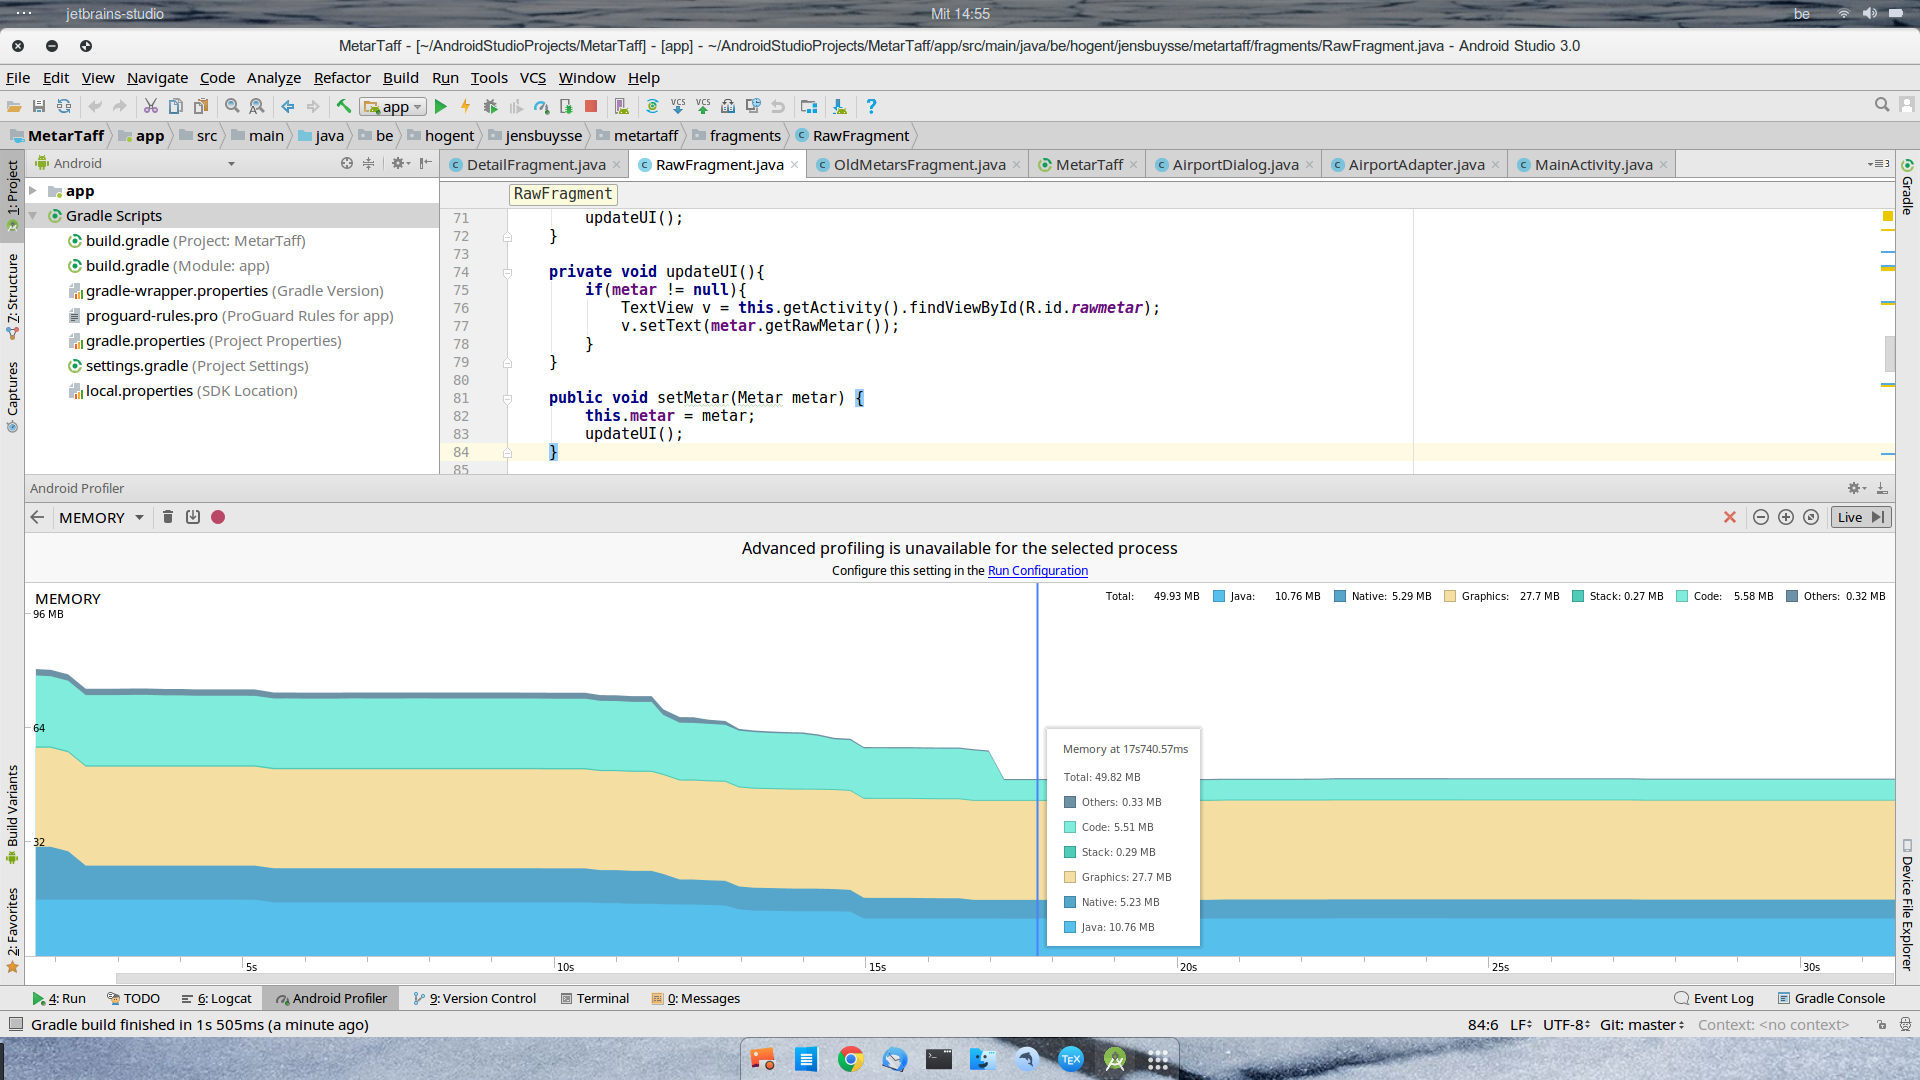
\includegraphics[width=\textwidth]{images/memory/profiler.png}
	\caption{Android provides a managed memory environment . When it determines that your app is no longer using some objects, the garbage collector releases the unused memory back to the heap}
	\label{fig:profiler}
\end{figure}

Explanation can be found \href{https://developer.android.com/studio/profile/memory-profiler.html}{here.}

\subsection{Leak Canary}
LeakCanary is an Open Source Java library to detect memory leaks in your debug builds. It is the canary in the coal mine for memory leaks: it detects memory leaks before any out-of-memory crashed are thrown. 

\section{Memory leaks: common leak patterns}
There are lots of ways you can cause a memory leak in Android. To summarize, there are mainly three categories.

\begin{enumerate}
	\item Leak activity to a static reference
	\item Leak activity to a worker thread
	\item Leak thread itself
\end{enumerate}

\subsection{Leak activity to a static reference}
A static reference lives as long as your app is in memory. An activity has lifecycles which are usually destroyed and re-created multiple times during you app’s lifecycle. If you reference an activity directly or indirectly from a static reference, the activity would not be garbage collected after it is destroyed. An activity can range from a few kilo bytes to many mega bytes depending on what contents are in it. If it has a large view hierarchy or high resolution images, it can make a large chunk of memory leaked.

\subsection{Leack activity to worker thread}
A worker thread can also out-live an Activity. If you reference an Activity directly or indirectly from a worker thread which lives longer than the Activity, you also leak the Activity object.

\subsection{Leak thread}
Every time you start a worker thread from an activity, you are responsible of managing the worker thread yourself. Because the worker thread can live longer than the Activity, you should stop the worker thread properly when the Activity is destroyed. If you forget to do so, you are risking leaking the worker thread itself.

These leaks are illustrated by \href{https://github.com/frank-tan/SinsOfMemoryLeaks}{Frank Tan}.

\newpage
\section{Exercises}
\begin{exercise}
	Add Leak Canary to the DotPict-, WhoIsIt and Metar application and find out if any of them suffer from memory leaks. If so, you should do the following things:
	\begin{itemize}
		\item Create a new branch where you fix the problem
		\item Document the memory leak by writing a short paragraph on how the leak got constructed, how you detected it and how you solved it. 
	\end{itemize}
	
\end{exercise}


\chapterimage{images/books.png}
\printbibliography

\printindex
\end{document}
